\documentclass{article}
\usepackage{iclr2021_conference,times}

\usepackage[utf8]{inputenc}
\usepackage[T1]{fontenc}
\usepackage{amsfonts}
\usepackage{microtype}
\usepackage{hyperref}
\usepackage{tikz}
\usetikzlibrary{arrows,decorations.pathmorphing,backgrounds,positioning,fit,petri}
\usepackage{booktabs}
\usepackage{graphicx}
%\usepackage[square,numbers]{natbib}
\usepackage{makecell}
\usepackage[ruled,vlined]{algorithm2e}
\usepackage{subcaption}

\usepackage{textcomp}
\usepackage{amsthm}
\usepackage{amsmath}

\newtheorem{thm}{Theorem}
\newtheorem{lem}{Lemma}

\newcommand{\nt}[1]{{\bf [#1]}}
\newcommand{\R}{\mathbb{R}}


\title{MeLES: Metric learning for event sequences with self-supervision}

\author{
Dmitrii Babaev \\
% dmitri.babaev@gmail.com
Sberbank AI Lab
\And
Ivan Kireev \\
Sberbank AI Lab
\And
Nikita Ovsov \\
Sberbank AI Lab
\And
Gleb Gusev \\
Sberbank AI Lab
\And
Maria Ivanova \\
Sberbank AI Lab
\And
Alexander Tuzhilin \\
% atuzhili@stern.nyu.edu
New York University
}

\begin{document}

\maketitle

\begin{abstract}

We address the problem of self-supervised learning on discrete event sequences generated by real-world users. Self-supervised learning incorporates complex information from the raw data in low-dimensional fixed-length vector representations that could be easily applied in various downstream machine learning tasks. In this paper, we propose a new method MeLES, which adopts metric learning, previously used for supervised tasks, to a self-supervised setting. It is based on a new theoretically justified algorithm, which provides surrogate positive pairs using sub-sequences from the raw data.

We evaluated MeLES on several public datasets and showed that MeLES representations outperform other methods on different downstream classification~tasks.

\end{abstract}

\section{Introduction} \label{sec-intro}

The size of the dataset is crucial for performance of modern supervised learning techniques~\cite{Sun2017RevisitingUE}. However, considering the rapid emergence of new applications and tasks in different domains, it is not possible to collect enough labeled data for many real world scenarios. This problem motivates extensive research~\cite{Tan2018ASO, Pan2010ASO} in the area of knowledge transfer where a model trained for one task can be further used as a good starting point for training in other tasks. A promising and rapidly growing approach is known as self-supervised learning\footnote{See, e.g., keynote by Yann LeCunn at ICLR-20: https://www.iclr.cc/virtual\_2020/speaker\_7.html}. The idea of self-supervised learning is to learn internal patterns of the input data based on a convenient synthetic task encouraging exploration without any additional information about "golden truth" output ~\cite{Peters2018DeepCW}, ~\cite{Devlin2019BERTPO},~\cite{Doersch2015UnsupervisedVR}, ~\cite{Oord2018RepresentationLW}. 
%Self-supervised learning is the main choice for pre-training in situations where the amount of labeled data for the target task of interest is very limited.

% Self-supervised learning has demonstrated great performance results in different machine learning domains, including that of Natural Language Processing (e.g., ELMO~\cite{Peters2018DeepCW}, BERT~\cite{Devlin2019BERTPO}) and computer vision~\cite{Doersch2015UnsupervisedVR}. There are also special self-supervised methods designed for continuous sequences, such as CPC~\cite{Oord2018RepresentationLW} for speech. However, 

There has been very little work on applicability of self-supervised learning to the discrete event sequences domain. One common example of discrete event sequences is user behavior sequences~\cite{Ni2018PerceiveYU} produced in many business applications including credit card transactions and click-stream data of online services. User behavior sequence is an event sequence that is attributed to a person and captures his/her regular and routine actions of certain type, e.g., transactions, search queries, phone calls and messages. The analysis of these sequences constitutes a very important field of machine learning~\cite{Laxman2008StreamPU, Wiese2009CreditCT, Zhang2017CreditRA, Bigon2019PredictionIV}.


In this paper, we propose \emph{MEtric Learning for Event Sequences (MeLES)} method that learns low-dimensional representations of discrete event sequences. This is the first self-supervised method proposed for discrete event sequences. It is based on a 
% In a broad sense, MeLES method
novel concept, which adopts the ideas of metric learning~\cite{Xing2002DistanceML, Hadsell2006DimensionalityRB}, used earlier for supervised tasks, to our self-supervised setting. The aim of metric learning is to represent semantically similar objects (images, video, audio, etc.) closer to each other, while dissimilar ones further away. Most of the metric learning methods are used in such applications as speech recognition~\cite{Wan2018GeneralizedEL}, computer vision~\cite{Schroff2015FaceNetAU, Mao2019MetricLF} and text analysis~\cite{Reimers2019SentenceBERTSE}. In these domains, metric learning is successfully applied in a supervised manner using pairs of high-dimensional instances that are labeled as the same (or similar) objects or different ones. MeLES is based on the observation that event sequences usually possess periodicity and repeatability of its events. We propose and theoretically justify a new algorithm, which generates sub-sequences of observed event sequences and uses them as different high-dimensional representations of the same object for metric learning.
%Therefore, one can consider some convenient sub-sequences of the same sequence as auxiliary high-dimensional representations of the same stochastic process that produced the observed sequence. By utilizing sub-sequence generation, it is possible to combine metric learning with self-supervision and get an algorithm that does not require labelling.
%MeLES model trained in a self-supervised manner can be used in two ways. Representations, produced by the model can be directly used as a fixed vector of features in some supervised downstream task (e. g. classification task) similarly to~\cite{Mikolov2013EfficientEO, Song2017LearningUE, Zhai2019LearningAU}. Alternatively, the trained model can be fine-tuned~\cite{Devlin2019BERTPO} for the specific downstream task.

We applied MeLES to several user behavior sequence~\cite{Ni2018PerceiveYU} datasets with different downstream classification tasks. When used directly as feature vectors, MeLES representations achieve strong performance comparable to hand-crafted features produces by data scientists with domain knowledge. Fine-tuned MeLES representations outperform supervised methods based on other representations by a significant margin. %Moreover, we show superiority of MeLES embeddings over the supervised approach applied to the partially labeled raw data due to insufficient amount of the target to learn a sufficiently complex model from scratch.
We provide the full source code for all the experiments described in the paper\footnote{https://github.com/***/*** (the link was anonymized for the double-blind peer review purposes)}.

Summing up, we make the following contributions: (1) we proposed the first self-supervised method for discrete event sequences; (2) we developed MeLES, which adopts the ideas of metric learning to self-supervised setting; (3) we demonstrated that the proposed MeLES method significantly outperforms previous approaches both in supervised and the semi-supervised learning scenarios. %on four different user behavior sequence datasets.

\section{Problem setting and background}\label{sec:problem setting}

While the idea proposed in this paper could be studied in different domains, we initially designed MeLES for discrete sequences of events. We assume that sequences of events $\{x_e(t)\}^{T_e}_{t=1}$ represent behavior of persons, or, more generally, life activity of some entities $e$. Events $x_e(t)$ may have any nature and structure (transactions of a client, click logs of a user), and their components may contain numerical, categorical and textual fields, see Section~\ref{sec-datasets}. Our goal is to learn an \textit{encoder} $M$ that maps sequences into a feature space~$\R^d$ in such a way that obtained \textit{embedding} $c_e=M(\{x_e(t) \})\in \R^d$ encodes essential properties of~$e$ and disregards any randomness and noise contained in sequence $\{x_e(t)\}^{T_e}_{t=1}$. The quality of representations can be examined by different downstream tasks related to the properties of entity $e$ in two ways. Representation $c_e$ can be used as a feature vector for a task--specific model, and encoder $M$ can be also (jointly) fine-tuned~\cite{Yosinski2014HowTA}.


%Sequence embedding $c_t$ obtained by the metric learning approach is then used in various downstream machine learning tasks as a feature vector. Also, a possible way to improve the downstream task performance is to feed a pre-trained embedding $c_t$ (e. g. the last layer of RNN) to a task-specific classification subnetwork and then jointly fine-tune the model parameters of the encoder and classifier subnetworks~\cite{Yosinski2014HowTA}.


In this paper, we make the first attempt to apply metric learning to this self-supervised setting. Previously, metric learning was successfully applied in a \textit{supervised} way in different domains (CV, speech, NLP, etc.), where the same \textit{person} or \textit{entity} can be represented by different \textit{samples}. We briefly review its general idea. Assume that each entity $e$ is associated with a probabilistic distribution $P_e$ over all possible samples (e.g., in face recognition, a person is a distribution over all his/her photos that can potentially appear in the life). The idea is to train encoder $M$ such that samples of the same or similar entities represented in the feature space are closer to each other than samples of different (dissimilar) entities. Mapping $M$ defines a pushforward $P_M(e):=M\#P_e$ of distribution $P_e$ in the feature space $\R^d$ for each entity $e$. In these terms, metric learning tends to separate distributions $P_M(e)$ of different entities $e$ as much as possible. The aim of previous literature on metric learning is to identify the entity based on its sample~\cite{Schroff2015FaceNetAU, Hu2014DiscriminativeDM, Wan2018GeneralizedEL}. Therefore, their training datasets naturally contain several independent samples per each particular entity, which form~\textit{positive pairs} (pairs of samples of the same entity) as a critical component for learning.


%One of the difficulties with applying a metric learning approach to the discrete event sequences is that the notion of semantic similarity as well as dissimilarity requires underlying domain knowledge and human labor-intensive labeling process to constrain positive and negative examples. 
On the contrary, our task is self-supervised, and we have no positive pairs. Instead, we have only one sequence per one entity. In the above formalism, each entity $e$ is associated with a distribution over event sequences, i.e., with a latent stochastic process $\{X_e(t)\}_{t=1}^{T_e}$. In this way, particular event sequence $\{x_e(t)\}_{t=1}^{T_e}$ that represents entity $e$ in the dataset is generated by this process $\{X_e(t)\}$. In the next section, we introduce a novel concept named MeLES, which allows to apply metric learning in the absence of positive pairs in the data.

\section{MeLES method} \label{sec-method}

\subsection{Sampling of surrogate sequences} \label{sec-pos-pairs}

If we had pairs of sample sequences generated by the same process $\{X_e(t)\}$, we could apply metric learning to our task. While we have no access to the latent process $\{X_e(t)\}$, we hope to generate \textit{surrogate} sequences as sub-sequences of the same event sequence $\{x_e(t)\}$ instead. The idea proposed below resembles the bootstrap method~\cite{Efron1994Bootstrap}, which enables to generate several bootstrap samples using only one sample of independent datapoints of a latent distribution. However, our setting is different, since we have no independent observations, so we should rely on different data assumptions. 


The key property of event sequences that represent life activity is periodicity and repeatability of the events in the stream. This is a motivation for the \textit{Random slices} sampling method applied in MeLES, see Algorithm~\ref{alg-slce-ss}. Each sub-sequence is generated from the initial sequence as its connected segment ("slice") in three steps. First, the length of the slice is chosen uniformly from possible values. Second, its starting position is uniformly chosen from all possible values. Third, too short (and optionally too long) sub-sequences are discarded. It could seem that the mean length of obtained sub-sequences are less than the mean length of sequences in the dataset. However, we show in the next section that the distribution of sub-sequences is close to the initial distribution in some realistic assumptions. The overview of the MeLES method is presented in Figure \ref{fig-arch}.


\begin{figure}[htbp]
  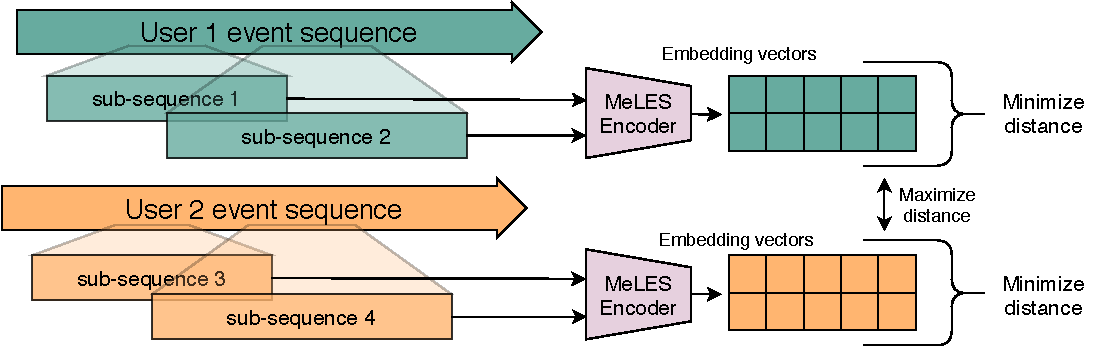
\includegraphics[width=\linewidth]{figures/arch-v2-narrow.pdf}
\caption{General framework}
  \label{fig-arch}
\end{figure}



\begin{algorithm}
\SetAlgoLined
\textbf{hyperparameters:} $m, M$: minimal and maximal possible length of a sub-sequence\\ $k$: number of trials.\\ %sub-sequences to be produced. \\
\textbf{input:} A sequence $S$ of length $T$. \\
\textbf{output:} $\mathcal{S}$: sub-sequences of $S$. \\

\BlankLine
 \For{$i\leftarrow 1$ \KwTo $k$}{
 Generate random integer $T_i$ uniformly from $[1,T];$\\
 \uIf{$T_i\in [m, M]$}
 {
  Generate random integer $s$ from $[0, T-T_i-1]$;\\
  Add $S_i := S[s: s + T_i-1]$ to $\mathcal{S}$
 }
}
\caption{Random slices sub-sample generation strategy}
\label{alg-slce-ss}
\end{algorithm}

\subsection{Theoretical analysis} \label{sec-theory}

Assume that process $\{X_e(t)\}_{t=1}^{T_e}$ is a segment of a latent process $\{\widehat{X}_e(t)\}_{t=1}^{\infty}$, which generates sequence of all events in the potentially infinite life of entity $e$. That is, we assume that $X_e(t)=\widehat{X}_e(t+s_e)$ for some random starting point $s_e\in \{0,1,\ldots\}$ and horizon $T_e$. Thus we observe, in our data, segment $[s_e+1,s_e+T_e]$ of the life of $e$. We also make the following Assumptions:
\begin{enumerate}
    \item Process $\{\widehat{X}_e(t)\}_{t=1}^{\infty}$ is cyclostationary (in the strict sense)~\cite{Gardner2006Cyclostationarity} with some period $\widehat{T}$.
    \item Starting $s_e$ is independent, and the distribution of $(s_e \mod \widehat{T})$ is uniform over $[0,\widehat{T}-1]$.
    \item Horizon $T_e$ is independent and follows a power--law distribution on $[m,\infty]$.
\end{enumerate}
These assumptions correspond to a scenario where potential clients or users can appear at a service at a random moment for some random horizon.    %First assumption is $\ldots$ 
\begin{thm}\label{thm:distribution}
If sequences $\{x_e(t)\}$ in the dataset are generated from latent processes $\{\widehat{X}_e(t)\}$ as described above, then sub-sequences obtained by Algorithm~\ref{alg-slce-ss} from $\{x_e(t)\}$ follow the same distribution as $\{x_e(t)\}$ up to a slight alteration of the distribution of the horizon $T_e$. Namely, if $T_e$ follows power law with an exponent $\alpha <-1$, then the density function for the length $T'_e$ of a sub-sequence satisfy $p(T'_e=k)/p(T_e=k)\in [(\frac{m-1}{m})^{-\alpha},(\frac{k}{k-1/2})^{-\alpha}]$.
\end{thm}
This theorem means that a sub-sequence obtained by Algorithm~\ref{alg-slce-ss} is a representative sample of entity~$e$. Further in this paper, we empirically examine whether pairs of such sub-sequences are useful for metric learning-based self-supervision. See Appendix~\ref{app-sec-proof} for the proof of Theorem~\ref{thm:distribution}.

\subsection{Batch generation}

The following procedure is used to create a batch during MeLES training. $N$ initial sequences are randomly taken for batch generation and $K$ sub-sequences are produced for each initial sequence. Pairs of sub-sequences produced from the same sequence are considered as positive samples and pairs from different sequences are considered as negative samples. Hence, after positive pair generation, each batch contains %$N \times K$ sub-sequences used as training samples. There are 
$NK(K-1)/2$ positive pairs and $K^2N(N - 1)/2$ negative pairs.

We consider several empirical strategies for sub-sequence generation to compare with Algorithm~\ref{alg-slce-ss}. The simplest strategy is the random sampling without replacement.
One more strategy is to produce sub-sequences by random splitting of the initial sequence to several connected segments without intersection between them
%To generate k sub-sequences, the following procedure should be repeated k times: take a random number of elements from the sequence \textit{without replacement}
(see Appendix~\ref{app-sec-bg}). The motivation is that intersections between sub-sequences may possibly lead to overfilling, since exact sub-sequences of events are the same and may be "remembered" without learning a deeper level of similarities.

% Note, that the order of events in generated sub-sequences is always preserved.


\subsection{Metric learning losses} \label{sec-ml-loss}

We consider several metric learning losses that showed promising performance on different datasets~\cite{Kaya2019DeepML} and some classical variants: contrastive~loss~\cite{Hadsell2006DimensionalityRB}, binomial deviance loss~\cite{Yi2014DeepML}, triplet loss \cite{Hoffer2015DeepML}, histogram~loss~\cite{Ustinova2016LearningDE}, and margin~loss~\cite{Manmatha2017SamplingMI}. Among them, contrastive loss showed best performance in experiments (see Appendix~\ref{app-sec-design}).

\textbf{Contrastive loss} has a contrastive term for negative pairs of embeddings, which penalizes the model only if the distance between embeddings of negative pair is less than a margin $m>0$:  
\begin{equation}
 \mathcal{L} = \sum_{i=1}^P \left[ (1-Y)\frac{1}{2}(D_W^i)^2 +Y*\frac{1}{2}\{max(0,m-D_W^i)\}^2 \right],
\end{equation}
where $P$ is the count of all pairs in a batch, $D_W^i$ is a distance function between embeddings in i-th labeled sample pair, $Y$ is a binary label identifying that samples in the pair are similar (or the same).
As proposed in~\cite{Hadsell2006DimensionalityRB}, we use euclidean distance function: $D_W^i = D(A,B) = \sqrt{\sum_i(A_i - B_i)^2}$.

\textbf{Pair distance calculation.} In order to select negative samples, we need to compute pair-wise distance between all possible pairs of embedding vectors of a batch. For the purpose of making this procedure more computationally effective we perform normalization of the embedding vectors, i.e. project them on a hyper-sphere of unit radius (see Appendix~\ref{app-sec-perf-opt}).


\textbf{Negative sampling} is a way to address the following challenge of the metric learning approach: using all pairs of samples can be inefficient: for example, some of the negative pairs are already distant enough, thus these pairs are not valuable for the training~\cite{SimoSerra2015DiscriminativeLO, Manmatha2017SamplingMI, Schroff2015FaceNetAU}. Hence, only a part of possible negative pairs in the batch are used during loss calculation. We compared most popular choices for negative sampling applied for MeLES, the results are shown in Table~\ref{tab-neg-sampl}.

\subsection{Encoder architecture} \label{sec-enc-arch}

To embed a sequence of events to the fixed-size vector we use the encoder network, which consists of two conceptual parts: the event encoder and the sequence encoder subnetworks.

\textbf{The event encoder} $e$ takes the set of attributes of a single event $x_t$ and outputs its representation in the latent space $Z \in \R^d$: $z_t = e(x_t)$.
The event encoder consists of the several embedding layers and batch normalization layers. Each embedding layer is used to encode each categorical attribute of the event. Batch normalization is applied to numerical attributes of the event. Finally, outputs of every embedding layer and batch normalization layer are concatenated to produce the latent representation $z_t$ of the single event.

\textbf{The sequence encoder} $s$ takes latent representations of the sequence of events: $ z_{1:T} = z_1, z_2, \cdots z_T $ and outputs the representation of the whole sequence $c_t$ in the time-step $t$: $ c_t = s(z_{1:t}) $.
Several approaches can be used to encode a sequence~\cite{Cho2014LearningPR, Vaswani2017AttentionIA} . In our experiments we use the recurrent network (RNN) similarly to~\cite{Sutskever2014SequenceTS}. The output produced for the last event is used to represent the whole sequence of events. In case of RNN the last output $h_t$ is a representation of the sequence.

\section{Experiments} \label{sec-exp}

\subsection{Datasets} \label{sec-datasets}

In our research we chose several publicly available datasets from data science competitions by means of sufficient amount of discrete events per user, hence, suitable for our method to obtain meaningful representations.
\newline \textbf{Age group prediction competition}\footnote{https://ods.ai/competitions/sberbank-sirius-lesson} - the dataset of 44M anonymized credit card transactions representing 50k persons was used to predict the age group of a person. Each transaction includes date, type and the amount being charged.
\newline \textbf{Gender prediction competition}\footnote{https://www.kaggle.com/c/python-and-analyze-data-final-project/} - the dataset of 6,8M anonymized card transactions representing 15K clients was used to predict a gender. Each transaction is characterized by date, type, amount and Merchant Category Code.
\newline \textbf{Assessment prediction competition}\footnote{https://www.kaggle.com/c/data-science-bowl-2019} - the task is to predict the in-game assessment results based on the history of children gameplay data. The dataset consists of 12M gameplay events representing 18k children. Each gameplay event is characterized by timestamp, event code, incremental counter of events within a game session, time since the start of the game session, etc.
\newline \textbf{Retail purchase history age group prediction}\footnote{https://ods.ai/competitions/x5-retailhero-uplift-modeling} - the task is to predict the age group of a client based on it retail purchase history. The dataset consists of 45,8M retail purchases representing 400k clients. Each purchase is characterized by time, product level, segment, amount, value, loyalty program points received.

\subsection{Experiment setup}

\textbf{Dataset split.} For each dataset, we set apart 10\% persons from the labeled part of the data as the test set that we used for comparing different models.
For all methods, random search on 5-fold cross-validation over the train set is used for hyper-parameter selection. The hyper-parameters with the best out-of-fold performance on train set are then chosen.
For evaluation of semi-supervised/self-supervised techniques (including MeLES), we used all transactions including unlabeled data, except for the test set, as far as those methods are suitable for partially labeled datasets, or does not require labels at all.

\textbf{Performance.} Neural network training was performed on a single Tesla P-100 GPU card. For the training part of MeLES, the single training batch is processed in 142 milliseconds. For example, in the age group prediction dataset the single training batch contains 64 unique persons with 5 sub-samples per person, i.e. 320 training samples in total, the mean number of transactions per sample is 90, hence each batch contains around 28800 transactions.

\subsubsection{Baselines} \label{sec-baselines}

%We compare our MeLES method with the following baselines.

\textbf{LightGBM.} We consider the Gradient Boosting Machine (GBM) method~\cite{Friedman2001GreedyFA} on hand-crafted features. GBM can be considered as a strong baseline in cases of tabular data with heterogeneous features. In particular, GBM-based approaches achieve the state-of-the-art results in a variety of practical tasks including web searches, weather forecasting, fraud detection, and many others~\cite{Wu2009AdaptingBF, Vorobev2019LearningTS, Zhang2015AGB, Niu2019ACS}.
GBM based model requires a large number of hand-crafted aggregate features produced from the raw transactional data. An example of an aggregate feature would be an average spending amount in some category of merchants, such as hotels of the entire transaction history.
We used LightGBM~\cite{Ke2017LightGBMAH} implementation of the GBM algorithm with nearly 1,000 hand-crafted features for the application. The companion code for the details of producing hand-crafted features can be found at ???.

\textbf{CPC.} As the second baseline, we selected the recently proposed Contrastive Predictive Coding (CPC)~\cite{Oord2018RepresentationLW}, a self-supervised learning method that produced excellent performance on sequential data of such traditional domains as audio, computer vision, natural language, and reinforcement learning. We adopted the CPC method to the discrete event sequences by making the model task to distinguish true future events from other types of events by using series of previous events as an input.

\textbf{Supervised learning}. In addition to the aforementioned baselines, we compare our method with a supervised learning approach where the encoder sub-network and the classification sub-network are jointly trained on the downstream task target. Note, that no pre-training is used in this case.

\subsubsection{Design choices} \label{sec-design}

Unless we explicitly specify, we use contrastive loss and random slices pair generation strategy in our experiments. We evaluated several possible loss choices and found that even contrastive loss that can be considered as the basic variant of metric learning loss, allows to get strong results on the downstream tasks (see Appendix~\ref{app-sec-design}). Our hypothesis is that an increase in model performance on the metric learning task does not necessarily lead to the performance increase on downstream tasks.

Furthermore, note that hard negative mining leads to significant increase in quality on downstream tasks in comparison to random negative sampling (see Table \ref{tab-neg-sampl}).

Another observation is that random slices sub-sequence generation strategy shows significantly better performance on the downstream tasks in comparison to the alternative strategies (see Table \ref{tab-pair-gen}) what confirm theoretical results (see Section \ref{sec-theory}).

The final set of hyper-parameters used for MeLES is shown in the Appendix~\ref{app-sec-exp-setup}.

\begin{table}
\centering
\caption{Comparison of batch generation strategies}
\begin{tabular}{llll}
\toprule
\textbf{Dataset} & \textbf{Random samples} & \textbf{Random disjoint samples} & \textbf{Random slices} \\
\midrule
\makecell{\textbf{Age group} \small{(Accuracy)}} & $0.593 \pm 0.003$ & $0.619 \pm 0.003$ & \textbf{0.642} $\pm 0.004$ \\
\makecell{\textbf{Gender} \small{(AUROC)}} & $0.857 \pm 0.005$ & $0.850 \pm 0.007$ & \textbf{0.882} $\pm 0.002$ \\
\makecell{\textbf{Assessment} \small{(Accuracy)}} & $0.546 \pm 0.004$ & $0.544 \pm 0.004$ & \textbf{0.604} $\pm 0.003$ \\
\makecell{\textbf{Retail} \small{(Accuracy)}} & $0.527 \pm 0.001$ & $0.526 \pm 0.001$ & \textbf{0.544} $\pm 0.001$ \\
\bottomrule
\end{tabular} \\
\small{5-fold cross-validation metric $\pm 95\%$ is shown}
\label{tab-pair-gen}
\end{table}

\begin{table}
\centering
\caption{Comparison of negative sampling strategies}
\begin{tabular}{llll}
\toprule
\textbf{Dataset} & \makecell{\textbf{Hard negative} \\ \textbf{mining}~\cite{Kaya2019DeepML}} & \makecell{\textbf{Random negative} \\ \textbf{sampling}} & \makecell{\textbf{Distance weighted} \\ \textbf{sampling}~\cite{Manmatha2017SamplingMI}} \\
\midrule
\makecell{\textbf{Age group} \small{(Accuracy)}} & \textbf{0.642} $\pm 0.004$ & $0.619 \pm 0.007$ & $0.628 \pm 0.005$ \\
\makecell{\textbf{Gender} \small{(AUROC)}} & \textbf{0.882} $\pm 0.002$ & $0.851 \pm 0.006$ & $0.878 \pm 0.001$ \\
\makecell{\textbf{Assessment} \small{(Accuracy)}} & \textbf{0.604} $\pm 0.003$ & $0.602 \pm 0.002$ & \textbf{0.604} $\pm 0.001$ \\
\makecell{\textbf{Retail} \small{(Accuracy)}} & \textbf{0.544} $\pm 0.001$ & $0.511 \pm 0.001$ & $0.514 \pm 0.001$ \\
\bottomrule
\end{tabular} \\
\small{5-fold cross-validation metric $\pm 95\%$ is shown}
\label{tab-neg-sampl}
\end{table}

\begin{figure}
  \centering
  \begin{minipage}[t]{0.49\linewidth}
    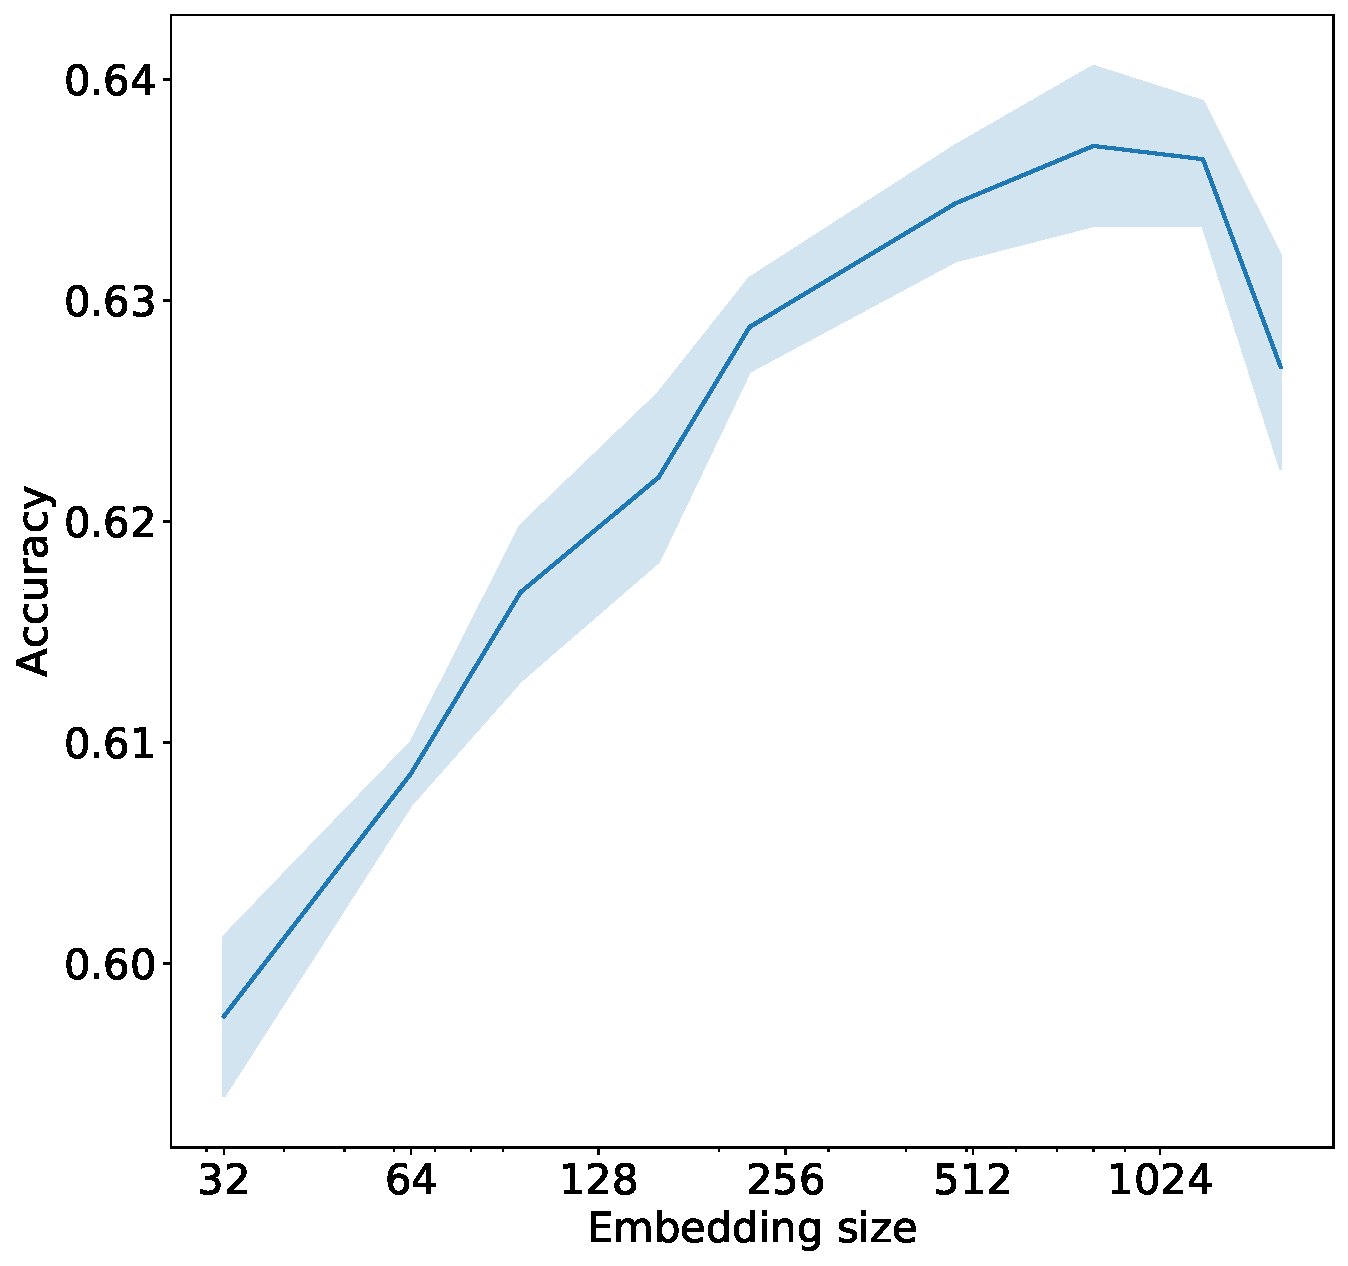
\includegraphics[width=\linewidth]{figures/age-pred-hidden-size.pdf}
    \caption{Embedding dimensionality vs. quality, age group prediction}
    \label{fig-emb-dim-age}
  \end{minipage}
  \hfill%
  \begin{minipage}[t]{0.49\linewidth}
    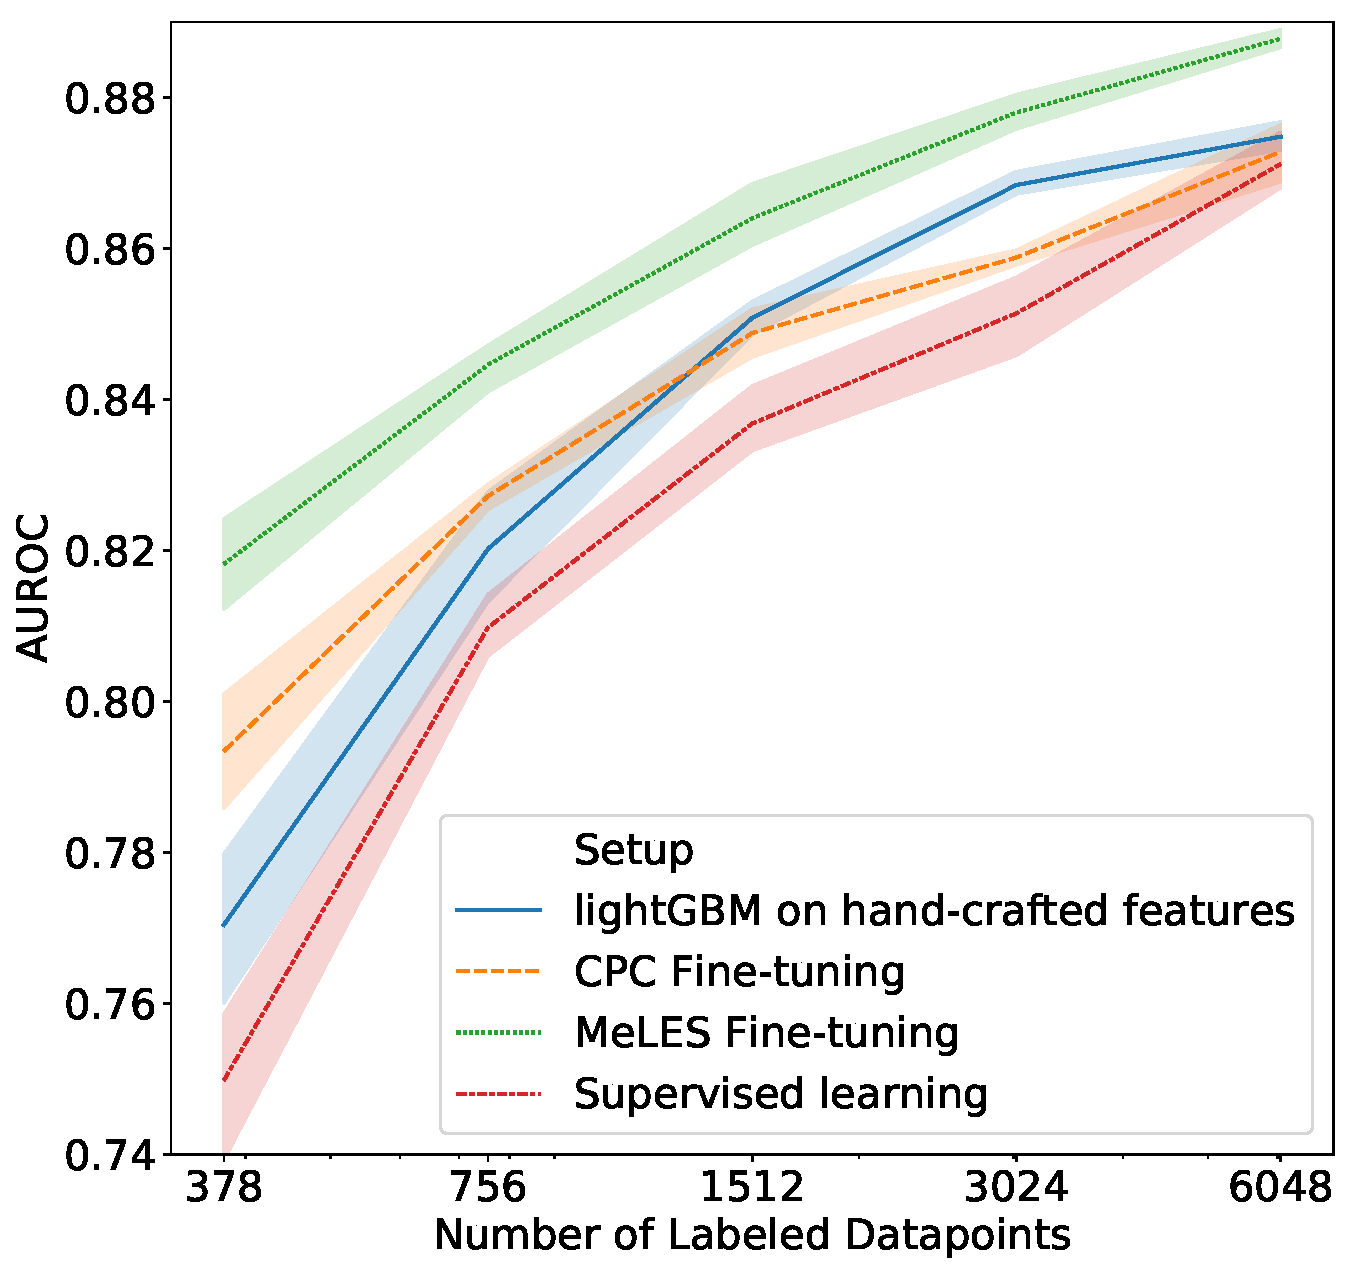
\includegraphics[width=\linewidth]{figures/ss_gen_4.pdf}
    \caption{Model quality for different dataset sizes, gender prediction}
    \small{The rightmost point correspond to all labels and supervised setup. X-axis is shown on a logarithmic scale.}
    \label{fig-semi-gender}
  \end{minipage}
\end{figure}

Figure \ref{fig-emb-dim-age} shows that the performance quality on the downstream task increases with  dimensionality of an embedding. The best quality is achieved at the size of 800. Further increase in  dimensionality of an embedding dramatically reduces quality.
These results can be interpreted as the bias-variance trade-off. When the embedding dimensionality is too small, too much information can be discarded (high bias). On the other hand, when embedding dimensionality is too large, too much noise is added (high variance).
Note, that increasing the embedding size will also linearly increase the training time and the volume of consumed memory on the GPU.

\subsection{Results} \label{sec-res}

\textbf{Comparison with baselines.} As Table \ref{tab-downstream-res} demonstrates, our method generates sequence embeddings of sequential data that achieve strong performance results in comparison to the case of manually crafted features when used on the downstream tasks. Moreover, fine-tuned representations obtained by our method achieve superior performance on all the considered datasets, outperforming all the previous learning methods by statistically significant margins.

\begin{table}
\centering
\caption{Accuracy on the downstream tasks: Metric increase against baseline}
\begin{tabular}{lllll}
\toprule
\textbf{Method} & \makecell{\textbf{Age group} \\ \small{Accuracy}} & \makecell{\textbf{Gender} \\ \small{AUROC}} &  \makecell{\textbf{Assessment} \\ \small{Accuracy}} & \makecell{\textbf{Retail} \\ \small{Accuracy}}\\
\midrule
\textbf{LightGBM:} \\
\makecell[r]{\textbf{Designed features}} & $0.632 \pm 0.005$ & $0.880 \pm 0.004$ & $0.591 \pm 0.003$ & $0.545 \pm 0.001$ \\
\makecell[r]{\textbf{CPC embeddings}} & $-6.0\% \pm  0.3\%$ & $-2.5\% \pm  0.2\%$ & $-1.2\% \pm  0.3\%$ & $-3.4\% \pm  0.1\%$\\
\makecell[r]{\textbf{\hspace{0.02\textwidth} MeLES embeddings}} & $1.6\% \pm  0.3\%$ & $0.3\% \pm  0.2\%$ & $2.2\% \pm  0.3\%$ & $-0.3\% \pm  0.1\%$ \\
\midrule
\textbf{Supervised learning} & $-0.6\% \pm  0.5\%$ & $-0.6\% \pm  0.3\%$ & $1.7\% \pm  0.3\%$  & $-0.6\% \pm  0.1\%$\\
\textbf{CPC fine-tuning} & $-1.8\% \pm  0.3\%$ & $-0.2\% \pm  0.2\%$ & $3.5\% \pm  0.4\%$ & $0.1\% \pm  0.2\%$ \\
\textbf{MeLES fine-tuning} & \textbf{1.0\%} $\pm  0.3\%$ & \textbf{1.9\%} $\pm  0.2\%$ & \textbf{3.9\%} $\pm  0.3\%$ & \textbf{0.7\%} $\pm  0.1\%$ \\
\bottomrule
\end{tabular} \\
\small{5-fold cross-validation metric $\pm 95\%$ is shown}
\label{tab-downstream-res}
\end{table}

\textbf{Semi-supervised setup.} To evaluate our method in case of the restricted amount of labeled data, we use only part of the available target labels for the semi-supervised experiment.
As in the case of the supervised setup, we compare the proposed method with LigthGBM over hand-crafted features, CPC, and supervised learning without pre-training (see Section \ref{sec-baselines}).

As Figure \ref{fig-semi-gender} shows, the difference in performance between MeLES and supervised-only methods increases as we decrease the number of available labels. Also note that MeLES consistently outperforms CPC for different volumes of labeled data.

\section{Related work} \label{sec-rel-work}

The widely used application fields of metric learning include computer vision~\cite{Chopra2005LearningAS},~\cite{Schroff2015FaceNetAU},  NLP~\cite{Reimers2019SentenceBERTSE} and audio~\cite{Wan2018GeneralizedEL}. Conventional metric learning methods incorporate some prior knowledge of the neighborhood relationships between the training samples by the means of explicitly labelling similar and dissimilar samples.

Inspired by performance advances in pretraining on a large unlabeled dataset and fine-tuning on a smaller labeled dataset, a novel self-supervised metric learning method (SimCLR)~\cite{Chen2020ASF} related to computer vision applications has been introduced recently. SimCLR proposes visual data augmentations to construct the training samples. Similar approach for computer vision is proposed in MoCo~\cite{He2019MomentumCF}. To the best of our knowledge, there are no self-supervised metric learning methods related to the discrete event sequence domain that have been previously proposed in the literature.

Another idea of applying self-supervised learning to non-discrete sequential data has been previously proposed in Contrastive Predictive Coding (CPC) method~\cite{Oord2018RepresentationLW}, where meaningful representations are extracted by predicting future in the latent space by using autoregressive methods. CPC representations demonstrated strong performance on four distinct domains: audio, computer vision, natural language and reinforcement learning. 

In the computer vision domain, there are many other than metric learning approaches related to self-supervised learning that are nicely summarized in~\cite{Jing2020SelfsupervisedVF}.
One of the common approaches to learn self-supervised representations is either traditional autoencoder~\cite{Rumelhart1986LearningIR} or variational autoencoder~\cite{Kingma2014AutoEncodingVB}. It is widely used for images, text and audio or aggregated event sequence data~\cite{Mancisidor2019LearningLR}. Although autoencoders have been successfully used in several domains listed above, they have not been applied to discrete event sequences either, mainly due to the challenges of defining distances between the input and the reconstructed input sequences.

There are papers dedicated to supervised learning on top of the discrete event sequences~\cite{Babaev2019ETRNNAD}, but self-superivized pre-training is not used in those papers.

\section{Conclusions} \label{sec-conclusions}

In this paper, we introduce \emph{Metric Learning for Event Sequences (MeLES)}, the first self-supervised method proposed for discrete event sequences.
In particular, the MeLES method can be effectively used for pre-training of neural networks in semi-supervised settings. It can also be used to produce embeddings of complex event sequences that can be effectively used in various downstream tasks.

We also empirically demonstrate that our approach achieves strong performance results on several downstream tasks by significantly outperforming both classical machine learning baselines on hand-crafted features, as well as other approaches based on self-supervision.
In the semi-supervised setting, where the number of labelled data is limited, our method demonstrates even stronger results: it outperforms supervised-only methods by larger margin as the number of labelled data decreases.

The proposed method of generating embeddings is convenient for production usage since the pre-calculated embeddings can be easily used for different downstream tasks without performing complex and time-consuming computations on the raw event data.
% For some encoder architectures, it is even possible to incrementally update the already calculated embeddings when new data arrives, as is shown in Section \ref{sec-perf-opt}.

% \section*{Broader Impact}

% This paper focused on developing a general novel metric learning method for the task of self-supervised learning for the discrete event sequences. Therefore, it can be applied to a broad range of practical applications, many of them having strong social and business impacts, such as educational applications dealing with logs of educational activities of  students, security applications dealing with logs of internet access activities and system logs protecting users from various types of malicious cyber-attacks, logs of online games, retail purchase histories, bank transactions and various other types of sequences. 

% Furthermore, our method has strong fairness mechanisms built into it since it focuses on the analysis of the granular event sequences and, therefore, does not have to deal with the problem of biased decisions and predictions stemming from poorly computed aggregate data leading to various types of social biases.

% Another advantage of using event sequence based embeddings, instead of the raw explicit event data, is that it is exceptionally difficult to restore the exact input sequence from its embeddings due to the fact, that lots of information is dropped during the transformation to embeddings. Therefore, the usage of embeddings leads to better privacy and data security for the end users than when working directly with the raw event data, and all this is achieved without sacrificing valuable information for downstream tasks.



\bibliographystyle{humannat}
\bibliography{neurips2020}

\appendix

\section{Batch generation} \label{app-sec-bg}

We consider several empirical strategies for sub-sequence generation to compare with random slices algorithm described in section "Sampling of surrogate sequences" of the main paper.
The simplest strategy is the random sampling without replacement.
One more strategy is to produce sub-sequences by random splitting of the initial sequence to several connected segments without intersection between them. To generate k sub-sequences, the following procedure should be repeated k times: take a random number of elements from the sequence \textit{without replacement}.

\begin{algorithm}
\SetAlgoLined
\textbf{hyperparameters:} $k$: number of sub-sequences to be produced. \\
\textbf{input:} A sequence $S$ of length $l$. \\
\textbf{output:} $S_1,...,S_k$: sub-sequences of $S$. \\

\BlankLine
Generate vector $inds$ of length $l$ with random integers from [1,k].\\
 \For{$i\leftarrow 1$ \KwTo $k$}{
 $S_i = S[inds == i]$
 }
\caption{Disjointed sub-sequences generation strategy}
\label{alg-disj-ss}

\end{algorithm}

\section{Performance optimizations} \label{app-sec-perf-opt}

Here we describe several performance optimizations that can be used for model training and inference.

\textbf{Pair distance calculation.} In order to select negative samples, we need to compute pair-wise distance between all possible pairs of embedding vectors of a batch. For the purpose of making this procedure more computationally effective we perform normalization of the embedding vectors, i.e. project them on a hyper-sphere of unit radius. Since $D(A,B) = \sqrt{\sum_i(A_i - B_i)^2} = \sqrt{\sum_i A_i^2 + \sum_i B_i^2 - 2\sum_i A_i B_i} $ and $||A||= ||B||=1$, to compute the euclidean distance we only need to compute: $\sqrt{2 - 2(A \cdot B)}$.

To compute the dot product between all pairs in a batch we just need to multiply the matrix of all embedding vectors of a batch by itself transposed, which is a highly optimized computational procedure in most modern deep learning frameworks. Hence, the computational complexity of the negative pair selection is $O(n^2h)$ where $h$ is the size of the output embeddings and $n$ is the size of the batch.

\textbf{Embedding update calculation.} Encoder, based on RNN-type architecture like GRU~\cite{Cho2014LearningPR}, allows to calculate embedding $c_{t+k}$ by updating embedding $c_t$ instead of  calculating embedding $c_{t+k}$ from the whole sequence of past events $z_{1:t}$: $c_k = rnn(c_t, z_{t+1:k})$. We use this optimization to reduce inference time to update already existing person embeddings with new events, occurred after the calculation of embeddings. This is possible due to the recurrent nature of RNN-like networks.

\section{Proof of Theorem 1} \label{app-sec-proof}

In this section, we provide the proof of Theorem 1 that justifies Random Slices sub-sequence generation strategy proposed in the paper. First, we give the statement of Theorem~1 for convenience.

Assume that process $\{X_e(t)\}_{t=1}^{T_e}$ is a segment of a latent process $\{\widehat{X}_e(t)\}_{t=1}^{\infty}$, which generates sequence of all events in the potentially infinite life of entity $e$. That is, we assume that $X_e(t)=\widehat{X}_e(t+s_e)$ for some random starting point $s_e\in \{0,1,\ldots\}$ and horizon $T_e$. Thus we observe, in our data, segment $[s_e+1,s_e+T_e]$ of the life of $e$. We also make the following Assumptions:
\begin{enumerate}
    \item Process $\{\widehat{X}_e(t)\}_{t=1}^{\infty}$ is cyclostationary (in the strict sense)~\cite{Gardner2006Cyclostationarity} with some period $\widehat{T}$.
    \item Starting $s_e$ is independent, and the distribution of $(s_e \mod \widehat{T})$ is uniform over $[0,\widehat{T}-1]$.
    \item Horizon $T_e$ is independent and follows a power--law distribution on $[m,\infty]$.
\end{enumerate}
\begin{thm}
If sequences $\{x_e(t)\}$ in the dataset are samples of processes $\{X_e(t)\}$, then sub-sequences obtained by the Random Slices generation strategy from $\{x_e(t)\}$ follow the same distribution as $\{x_e(t)\}$ up to a slight alteration of the distribution of the horizon $T_e$. Namely, if $T_e$ follows power law with an exponent $\alpha <-1$, then the density function for the length $T'_e$ of a sub-sequence satisfy 
\begin{equation}\label{probability_ratio}
\P(T'_e=k)/\P(T_e=k)\in \left [\left (\frac{m-1}{m}\right )^{-\alpha},\left (\frac{k}{k-1/2}\right )^{-\alpha}\right ].    
\end{equation}

\end{thm}

\begin{proof}
First, we state the following straightforward lemma:
\begin{lem}\label{stationary}
Let a stochastic process $\{Y(t)\}_{t=1}^{\infty}$ be a shift of another stochastic process $\{\widehat{Y}(t)\}_{t=1}^{\infty}$ by independent random time $s$, i.e. $Y(t) = \widehat{Y}(t+s)$ with integer $s\geq 0$. If process $\{\widehat{Y}(t)\}_{t=1}^{\infty}$ is cyclostationary with period $\widehat{T}$ and $(s_e \mod \widehat{T})$ is uniform over $[0,\widehat{T}-1]$, then process $\{Y(t)\}_{t=1}^{\infty}$ is stationary.
\end{lem}
Lemma~\ref{stationary} implies that process $\{X_e(t)\}_{t=1}^{T_e}$ is stationary, and all its segments $\{X_e(t)\}_{t=s'+1}^{T'_e+s'}$ of a given length $T'_e$ define the same distribution over sequences as its starting segment $\{X_e(t)\}_{t=1}^{T'_e}$ does. Furthermore, integrating over $s'$, we conclude that the conditional distribution of a sub-sequence obtained via Random Slices generation strategy given its length $T'_e$ follows the process $\{X_e(t)\}_{t=1}^{T'_e}$. To finish the proof, it remains to prove Equation~\ref{probability_ratio}.

Assume $\P(T_e=k)\propto k^{\alpha}$ for $k\in [m,\infty]$. By the law of total probability, we have $\P(T'_e=k_0)= \sum_{k}\P(T_e=k)\P(T'_e=k_0\mid T_e=k)$, that is,
$$
\P(T'_e=k_0) = C \sum_{k=k_0}^{\infty} k^{\alpha-1},
$$
where $C$ is the normalization constant. To estimate the sum of the series, notice that
\begin{equation}\label{int_inequal}
\int_{k_0-\frac{1}{2}}^\infty x^{\alpha-1} dx > \sum_{k=k_0}^{\infty} k^{\alpha-1} > \int_{k_0}^\infty x^{\alpha-1} dx,    
\end{equation}
where the former inequality follows from the fact that $\int_{k-1/2}^{k+1/2} x^{\alpha-1}> k^{\alpha-1}$ as long as function $f(x)=x^{\alpha-1}$ is convex. After integration, we rewrite Equation~\ref{int_inequal} as follows:
\begin{equation}\label{inequal}
\frac{-1}{\alpha} \left ( k_0-\frac{1}{2}\right )^{\alpha} > \sum_{k=k_0}^{\infty} k^{\alpha-1} > \frac{-1}{\alpha} k_0^{\alpha}. \end{equation}
Using these inequalities, we obtain the upper bound for $\P(T'_e=k)/\P(T_e=k)$ in the following way:
\begin{multline*}
\P(T'_e=k_0) = \sum_{k=k_0}^{\infty} k^{\alpha-1} / \sum_{l=m}^\infty \sum_{k=l}^{\infty} k^{\alpha-1} < \frac{-1}{\alpha} \left ( k_0-\frac{1}{2}\right )^{\alpha} / \sum_{l=m}^\infty \frac{-1}{\alpha} l^{\alpha} = \\
=\left (\frac{k_0}{k_0-1/2}\right )^{-\alpha} k_0^\alpha/\sum_{l=m}^\infty l^{\alpha} = \left (\frac{k_0}{k_0-1/2}\right )^{-\alpha} \P(T_e=k_0).
\end{multline*}
At last, the lower bound for $\P(T'_e=k)/\P(T_e=k)$ can be obtained using Equation~\ref{inequal} as follows:
\begin{multline*}
\P(T'_e=k_0) = \sum_{k=k_0}^{\infty} k^{\alpha-1} / \sum_{l=m}^\infty \sum_{k=l}^{\infty} k^{\alpha-1} > k_0^{\alpha} / \sum_{l=m}^\infty  \left (l-\frac{1}{2}\right )^{\alpha} > \\
> \left (\frac{m-1/2}{m}\right )^{-\alpha} k_0^\alpha/\sum_{l=m}^\infty l^{\alpha} = \left (\frac{m-1/2}{m}\right )^{-\alpha} \P(T_e=k_0).
\end{multline*}
The latter inequality in these calculations follows from the fact that $\left (\frac{l-\frac{1}{2}}{l}\right )^{\alpha}<\left (\frac{m-\frac{1}{2}}{m}\right )^{\alpha}$ for $l>m$.

\end{proof}

\section{Datasets} \label{app-sec-datasets}

We designed the method specially for the user behavior sequences~\cite{Ni2018PerceiveYU}. That sequences consist of discrete events per person in continuous time, for example,  behavior on websites, credit card transactions, etc. 

Considering credit card transactions, each transaction have a set of attributes, either categorical or numerical including the timestamp of the transaction. An example of the sequence of three transactions with their attributes is presented in the Table \ref{tab-tr-data}.
Merchant type field represents the category of a merchant, such as "airline", "hotel", "restaurant", etc.

\begin{table}
\centering
\caption{Data structure for a single credit card}
\begin{tabular}{llllll}
\toprule
\textbf{Date} & \textbf{Time} & \textbf{Amount} & \textbf{Currency} & \textbf{Country} & \textbf{Merchant Type} \\
\midrule
Jun 21 & 16:40& 230 & EUR & France & Restaurant \\
Jun 21 & 20:15 & 5 & USD & US & Transportation \\
Jun 22 & 09:30 & 40 & USD & US & Household Appliance \\
\bottomrule
\end{tabular}
\label{tab-tr-data}
\end{table}

Another example of user behavior data is click-stream: the log of internet pages  visits. The example of a click-stream log of a single user is presented in Table \ref{tab-cs-data}.

\begin{table}
\centering
\caption{Click-stream structure for a single user}
\begin{tabular}{llll}
\toprule
\textbf{Time} & \textbf{Date} & \textbf{Domain} & \textbf{Referrer Domain} \\
\midrule
17:40 & Jun 21 & amazon.com & google.com \\
17:41 & Jun 21 & amazon.com & amazon.com \\
17:45 & Jun 21 & en.wikipedia.org & google.com \\
\bottomrule
\end{tabular}
\label{tab-cs-data}
\end{table}


In our research we chose several publicly available datasets from data science competitions.
\begin{enumerate}
    \item \textbf{Age group prediction competition}\footnote{https://onti.ai-academy.ru/competition} - the task is to predict the age group of a person. The dataset consists of 44M anonymized transactions representing 50k persons with a target labeled for only 30k of them (27M out of 44M transactions), for the other 20k persons (17M out of 44M transactions) label is unknown. Each transaction includes date, type (for example, grocery store, clothes, gas station, children's goods, etc.) and amount. We use all available 44M transactions for metric learning, excluding 10\% - for the test part of the dataset, and  5\% for the metric learning validation.
        
    \item \textbf{Gender prediction competition}\footnote{https://www.kaggle.com/c/python-and-analyze-data-final-project/} - the task is a classification problem of predicting a gender. The dataset consists of 6,8M anonymized card transactions representing 15k clients, where only 8,4k of them are labeled. Each transaction is characterized by date, type (for ex. "ATM cash deposit"), amount and Merchant Category Code (MCC).
    
    \item \textbf{Assessment prediction competition}\footnote{https://www.kaggle.com/c/data-science-bowl-2019} - the task is to predict the in-game assessments results based on the history of children gameplay data. The dataset consists of 12M gameplay events representing 4,6k children. Each gameplay event is characterized by timestamp, event code, incremental counter of events within a game session, time since the start of the game session, etc.
    
    \item \textbf{Retail purchase history age group prediction}\footnote{https://ods.ai/competitions/x5-retailhero-uplift-modeling} - the task is to predict the age group of a client based on it retail purchase history. The dataset consists of ???M retail purchases representing ???k clients. Each purchase is characterized by time, product level, segment, amount, value, points received.

\end{enumerate}

\section{Experiment setup} \label{app-sec-exp-setup}

For all methods, random search on 5-fold cross-validation over the train set is used for hyper-parameter selection. The hyper-parameters with the best out-of-fold performance on train set are then chosen. The final set of hyper-parameters used for MeLES is shown in Table \ref{tab-hyper}.

\begin{table}
\centering
\caption{Hyper-parameters for MeLES training}
\begin{tabular}{lllllll}
\toprule
\textbf{Dataset} & \makecell[l]{\textbf{Learning} \\ \textbf{rate}} & \makecell[l]{\textbf{N samples} \\ \textbf{in batch}} & \textbf{N epochs} & \makecell[l]{\textbf{N} \\ \textbf{sub-samples}} & \makecell[l]{\textbf{Min seq} \\ \textbf{length}} & \makecell[l]{\textbf{Max seq} \\ \textbf{length}} \\
\midrule
\textbf{Age group} & 0.002 & 64 & 100 & 5 & 25 & 100 \\
\textbf{Gender} & 0.002 & 128 & 150 & 5 & 25 & 100 \\
\textbf{Assessment} & 0.002 & 256 & 100 & 5 & 100 & 500 \\
\textbf{Retail} & 0.002 & 256 & 30 & 5 & 30 & 180 \\
\bottomrule
\end{tabular}
\label{tab-hyper}
\end{table}

\subsection{Hand-crafted features} \label{app-sec-hand}

Here we describe the the details of producing hand-crafted features. All attributes of each transaction are either numerical (e. g. amount) or categorical (e.g. merchant type (MCC code), transaction type, etc.). 
For numerical type of attribute we apply aggregation functions, such as 'sum', 'mean', 'std', 'min', 'max', over all transactions per user. For example, if we apply 'sum' for the numerical field 'amount' we obtain a feature 'sum of all transaction amounts per user'. 
For categorical type of attribute we apply aggregation functions in a slightly different way. For each unique value of categorical attribute we apply aggregation functions, such as 'count', 'mean', 'std' over all transactions per user' numerical attribute. For example, if we apply 'mean' for the numerical attribute 'amount' grouped by categorical attribute 'mcc code' we obtain a feature 'mean amount of all transaction for each mcc code per user'. 
For example, for age prediction task we have one categorical attribute (small group) with 200 unique values, combining it with amount we can produce $200 * 3$ features ('group0 x amount x count',  'group1 x amount x count', ..., 'group199 x amount x count', 'group0 x amount x mean', ...). In total we use approx 605 features for age prediction task. For gender prediction task we have two categorical features: 'MCC code' with approx 200 unique values and 'tr type' with approx 100 unique values. So in total we use $200 * 3 + 100 * 3 + 5 = 905$ features.
Note, that hand-crafted features contain information about user spending profile but omit information about transactions temporal order.

\subsection{Design choices} \label{app-sec-design}

In the Table \ref{tab-enc-type} and Table \ref{tab-loss-type} we present the results of experiments on different design choices of our method.

As shown in Table \ref{tab-enc-type}, different choices of encoder architectures show comparable performance on the downstream tasks.

It is interesting to observe that even contrastive loss that can be considered as the basic variant of metric learning loss allows to get strong results on the downstream tasks (see Table \ref{tab-loss-type}). Our hypothesis is that an increase in the model performance on metric learning task does not always lead to an increase in performance on downstream tasks.

\begin{table}
\centering
\caption{Comparison of encoder types}
\begin{tabular}{llll}
\toprule
\textbf{Dataset} & \textbf{LSTM} & \textbf{GRU} & \textbf{Transformer} \\
\midrule
\textbf{Age group} \small{(Accuracy)} & 0.616 $\pm 0.006$ & \textbf{0.642} $\pm 0.004$ & $0.633 \pm 0.007$ \\
\textbf{Gender} \small{(AUROC)} & $0.866 \pm 0.003$ & \textbf{0.882} $\pm 0.002$ & $0.864 \pm 0.004$  \\
\textbf{Assessment} \small{(Accuracy)} & $0.601 \pm 0.003$ & \textbf{0.604} $\pm 0.003$ & $0.542 \pm 0.002$  \\
\textbf{Retail} \small{(Accuracy)} & $0.540 \pm 0.001$ & \textbf{0.542} $\pm 0.002$ & $0.503 \pm 0.001$  \\
\bottomrule
\end{tabular} \\
\small{5-fold cross-validation metric $\pm 95\%$ is shown}
\label{tab-enc-type}
\end{table}

\begin{table}
\centering
\caption{Comparison of metric learning losses}
\begin{tabular}{llllll}
\toprule
\textbf{Dataset} & \textbf{Contrastive} & \makecell{\textbf{Binomial} \\ \textbf{deviance}} & \textbf{Histogram} & \textbf{Margin} & \textbf{Triplet} \\
\midrule
\makecell{\textbf{Age group} \\ \small{(Accuracy)}} & \makecell{\textbf{0.642} \\ $\pm 0.004$} & \makecell{0.626 \\ $\pm 0.005$} & \makecell{0.629 \\ $\pm 0.004$} & \makecell{0.635 \\ $\pm 0.006$} & \makecell{0.637 \\ $\pm 0.002$} \\
\makecell{\textbf{Gender} \\ \small{(AUROC)}} & \makecell{\textbf{0.881} \\ $\pm 0.004$} & \makecell{0.861 \\ $\pm 0.004$} & \makecell{0.866 \\ $\pm 0.004$} & \makecell{\textbf{0.882} \\ $\pm 0.002$} & \makecell{0.860 \\ $\pm 0.005$} \\
\makecell{\textbf{Assessment} \\ \small{(Accuracy)}} & \makecell{\textbf{0.604} \\ $\pm 0.003$} & \makecell{0.576 \\ $\pm 0.004$} & \makecell{\textbf{0.608} \\ $\pm 0.001$} & \makecell{0.593 \\ $\pm 0.002$} & \makecell{0.601 \\ $\pm 0.003$} \\
\makecell{\textbf{Retail} \\ \small{(Accuracy)}} & \makecell{\textbf{0.542} \\ $\pm 0.002$} & \makecell{0.538 \\ $\pm 0.002$} & \makecell{0.538 \\ $\pm 0.001$} & \makecell{\textbf{0.546} \\ $\pm 0.002$} & \makecell{0.536 \\ $\pm 0.002$} \\
\bottomrule
\end{tabular} \\
\small{5-fold cross-validation metric $\pm 95\%$ is shown}
\label{tab-loss-type}
\end{table}

Figure \ref{fig-emb-dim} shows that the performance quality on the downstream task increases with dimensional of an embedding. As we can see the plots for different datasets have similar shape with significant drop after reaching the peak. As mentioned in the section "Design choices" of the main paper the possible reason of this drop is overfitting, i. e. embedding dimension does not serve as effective information bottleneck.

\begin{figure}
  \centering
  \caption{Embedding dimensionality vs. quality}
  \begin{subfigure}{0.5\linewidth}
    \caption{Age group prediction}
    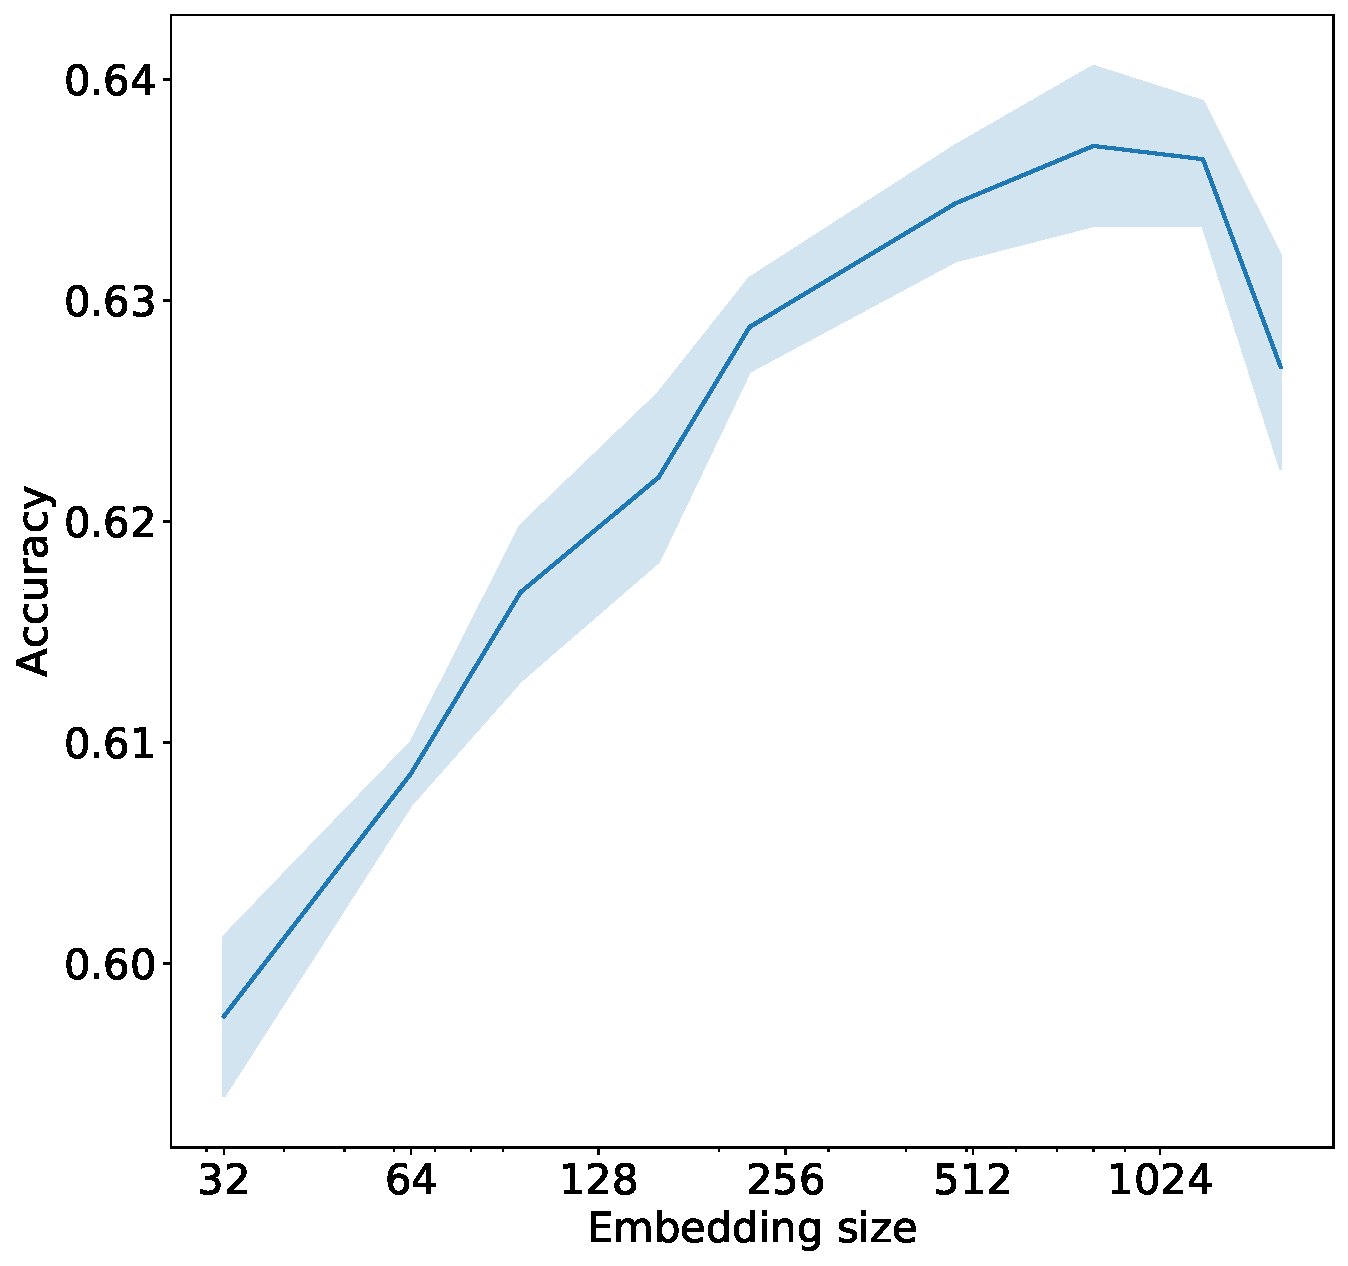
\includegraphics[width=\linewidth]{figures/age-pred-hidden-size.pdf}
  \end{subfigure}%
  \begin{subfigure}{0.5\linewidth}
    \caption{Gender prediction}
    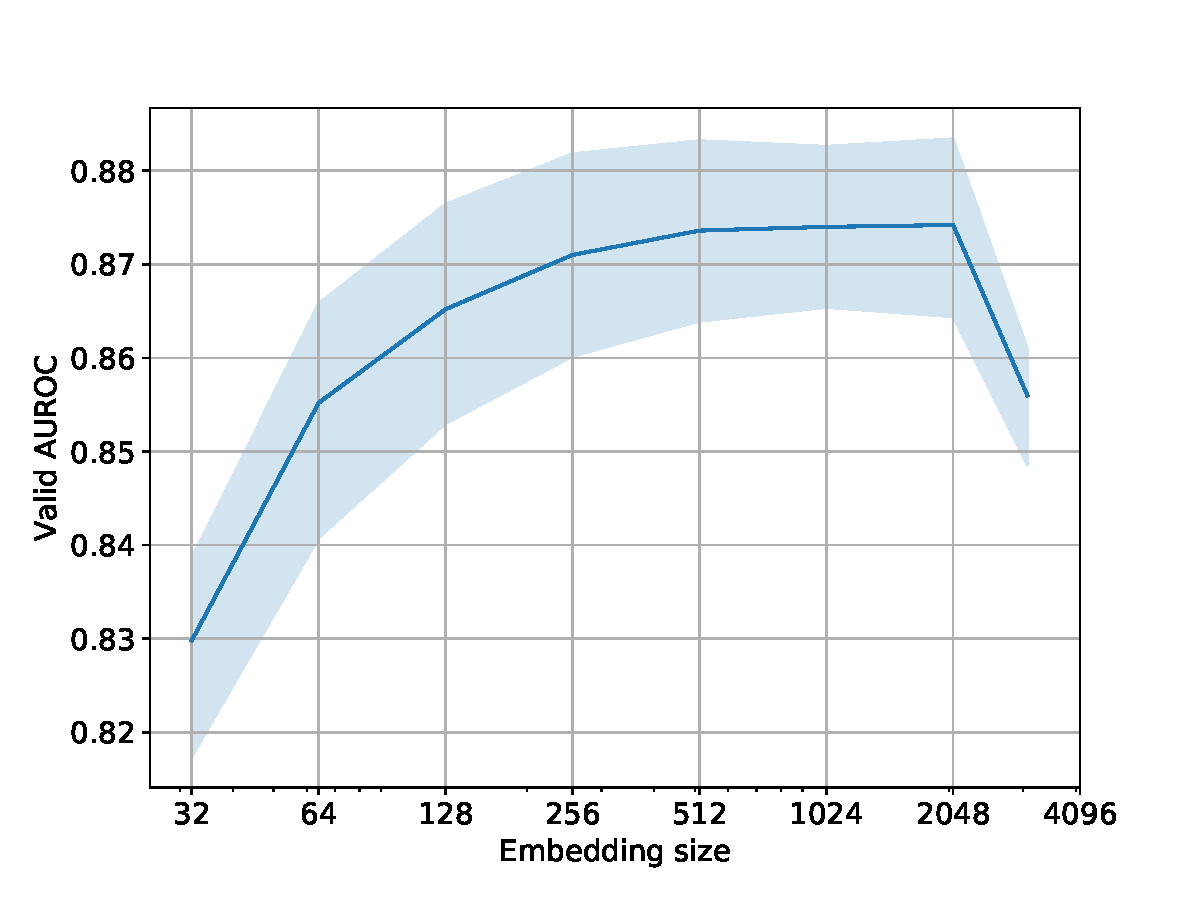
\includegraphics[width=\linewidth]{figures/gender-hidden-size.pdf}
  \end{subfigure}
  \begin{subfigure}{0.5\linewidth}
    \caption{Assessment prediction}
    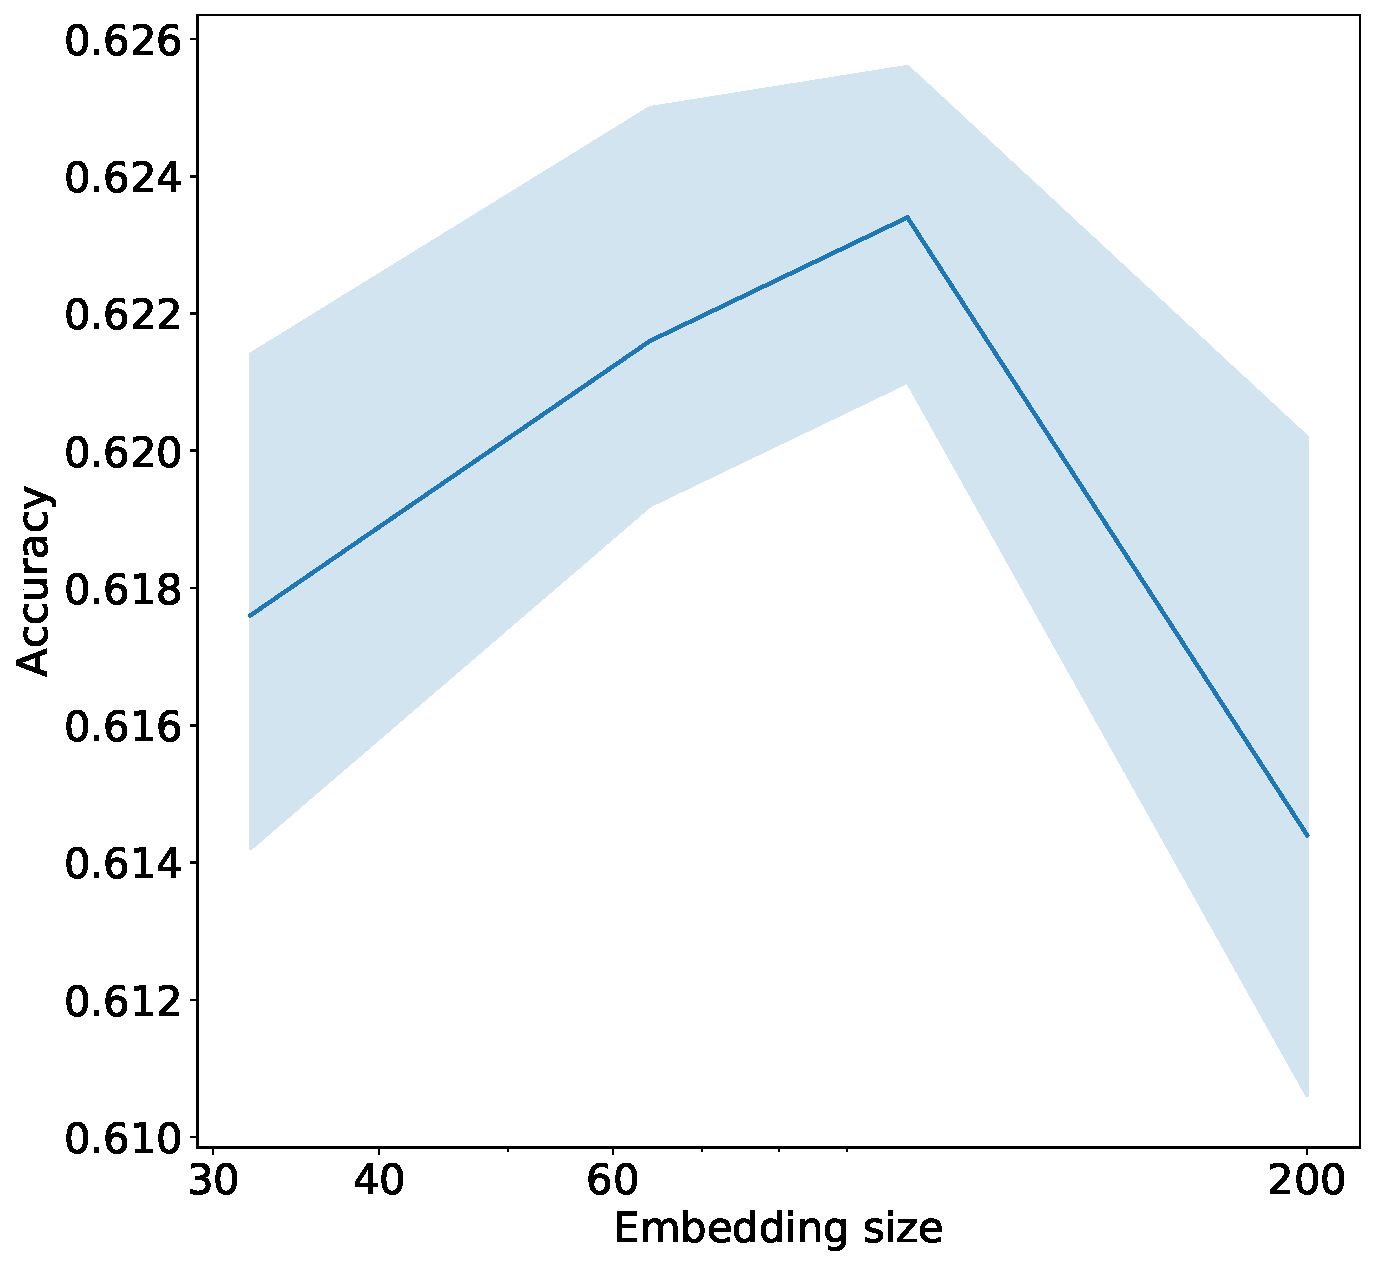
\includegraphics[width=\linewidth]{figures/bowl-hidden-size.pdf}
  \end{subfigure}%
  \begin{subfigure}{0.5\linewidth}
    \caption{Retail prediction}
    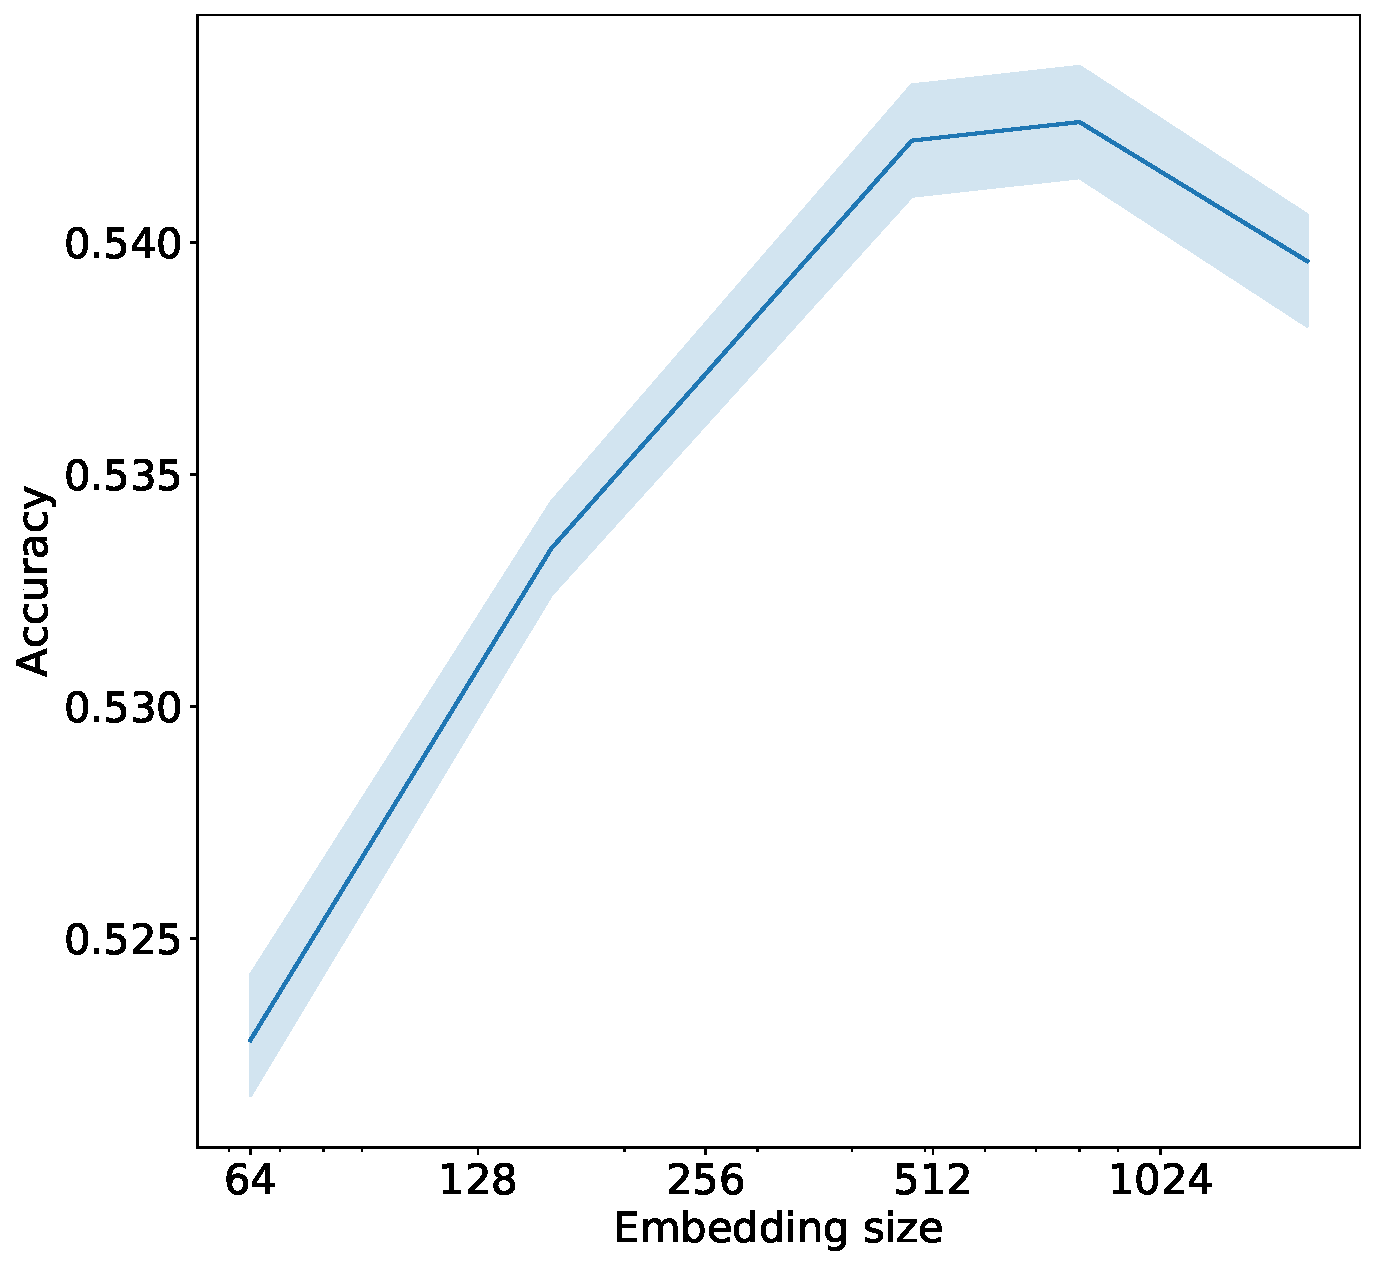
\includegraphics[width=\linewidth]{figures/x5-hidden-size.pdf}
  \end{subfigure}
  \label{fig-emb-dim}
\end{figure}

\section{Results} \label{app-sec-res}

\subsection{Semi-supervised setup} \label{app-sec-semi}

To evaluate our method in case of the restricted amount of labeled data, we use only part of the available target labels for the semi-supervised experiment. As in the case of the supervised setup, we compare the proposed method with LigthGBM over hand-crafted features, CPC, and supervised learning without pre-training. In figure \ref{fig-semi} we provide learning curves for all considered datasets.

\begin{figure}
  \centering
  \begin{subfigure}{0.5\linewidth}
    \caption{Age group prediction}
    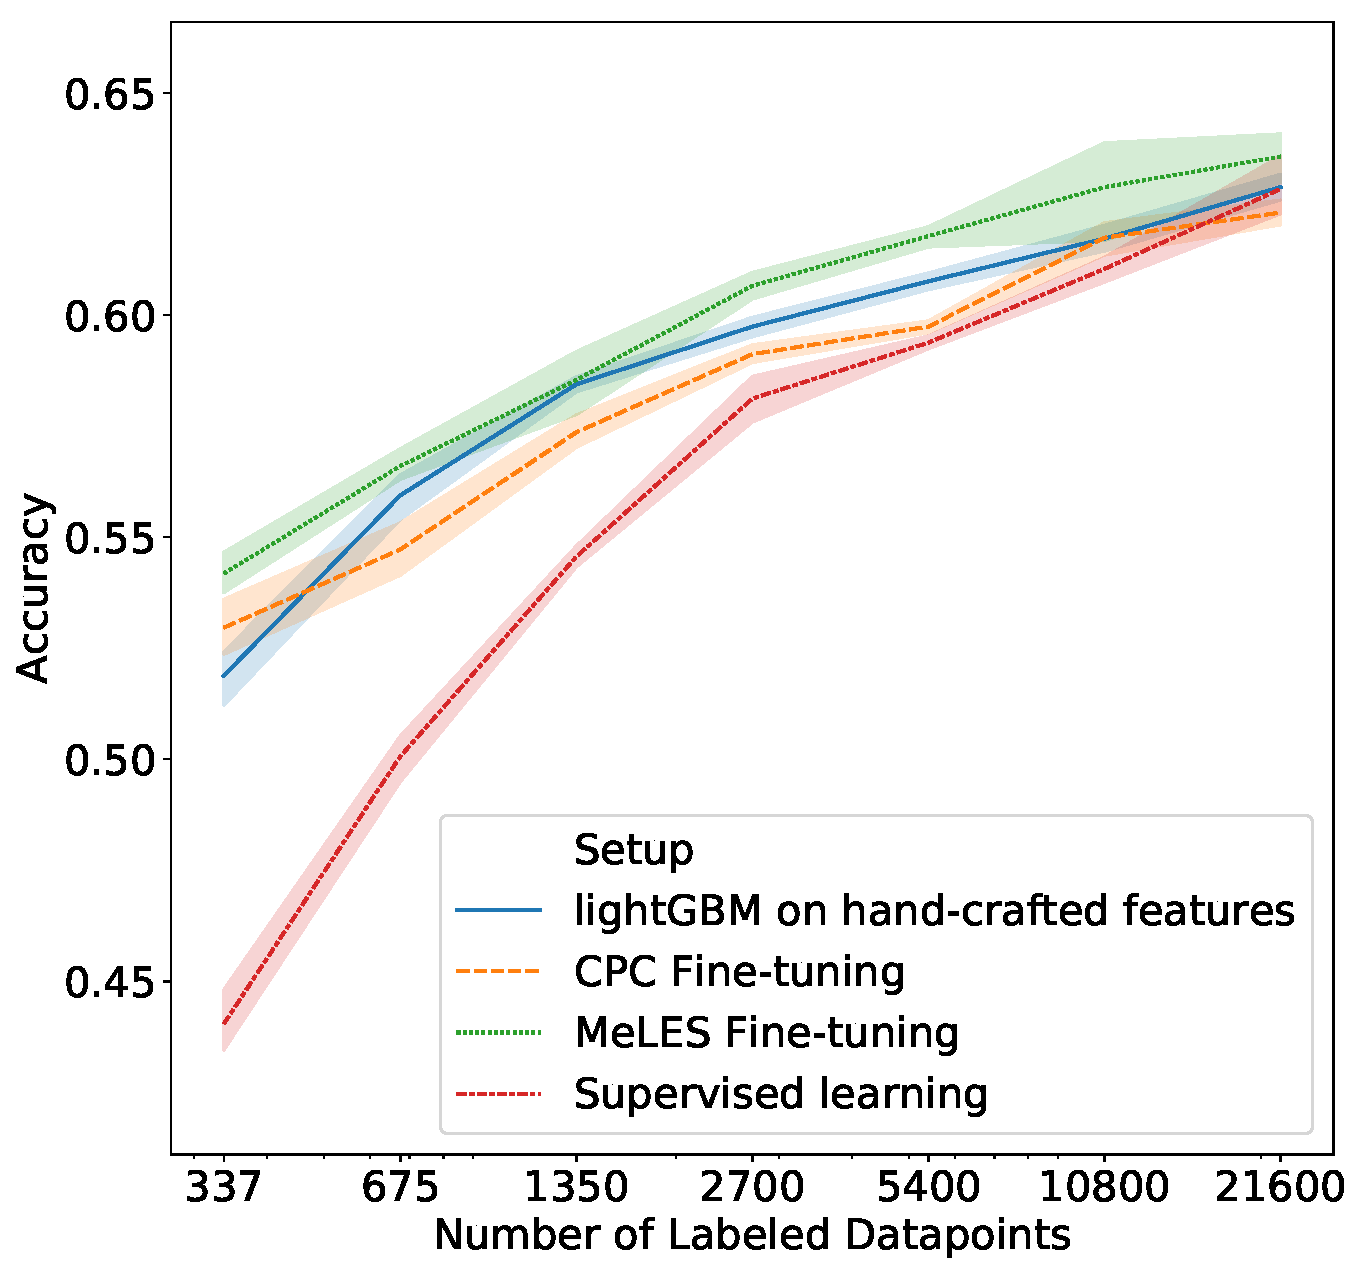
\includegraphics[width=\linewidth]{figures/ss_age_pred.pdf}
    \label{fig-semi-age-0}
  \end{subfigure}%
  \begin{subfigure}{0.5\linewidth}
    \caption{Gender prediction}
    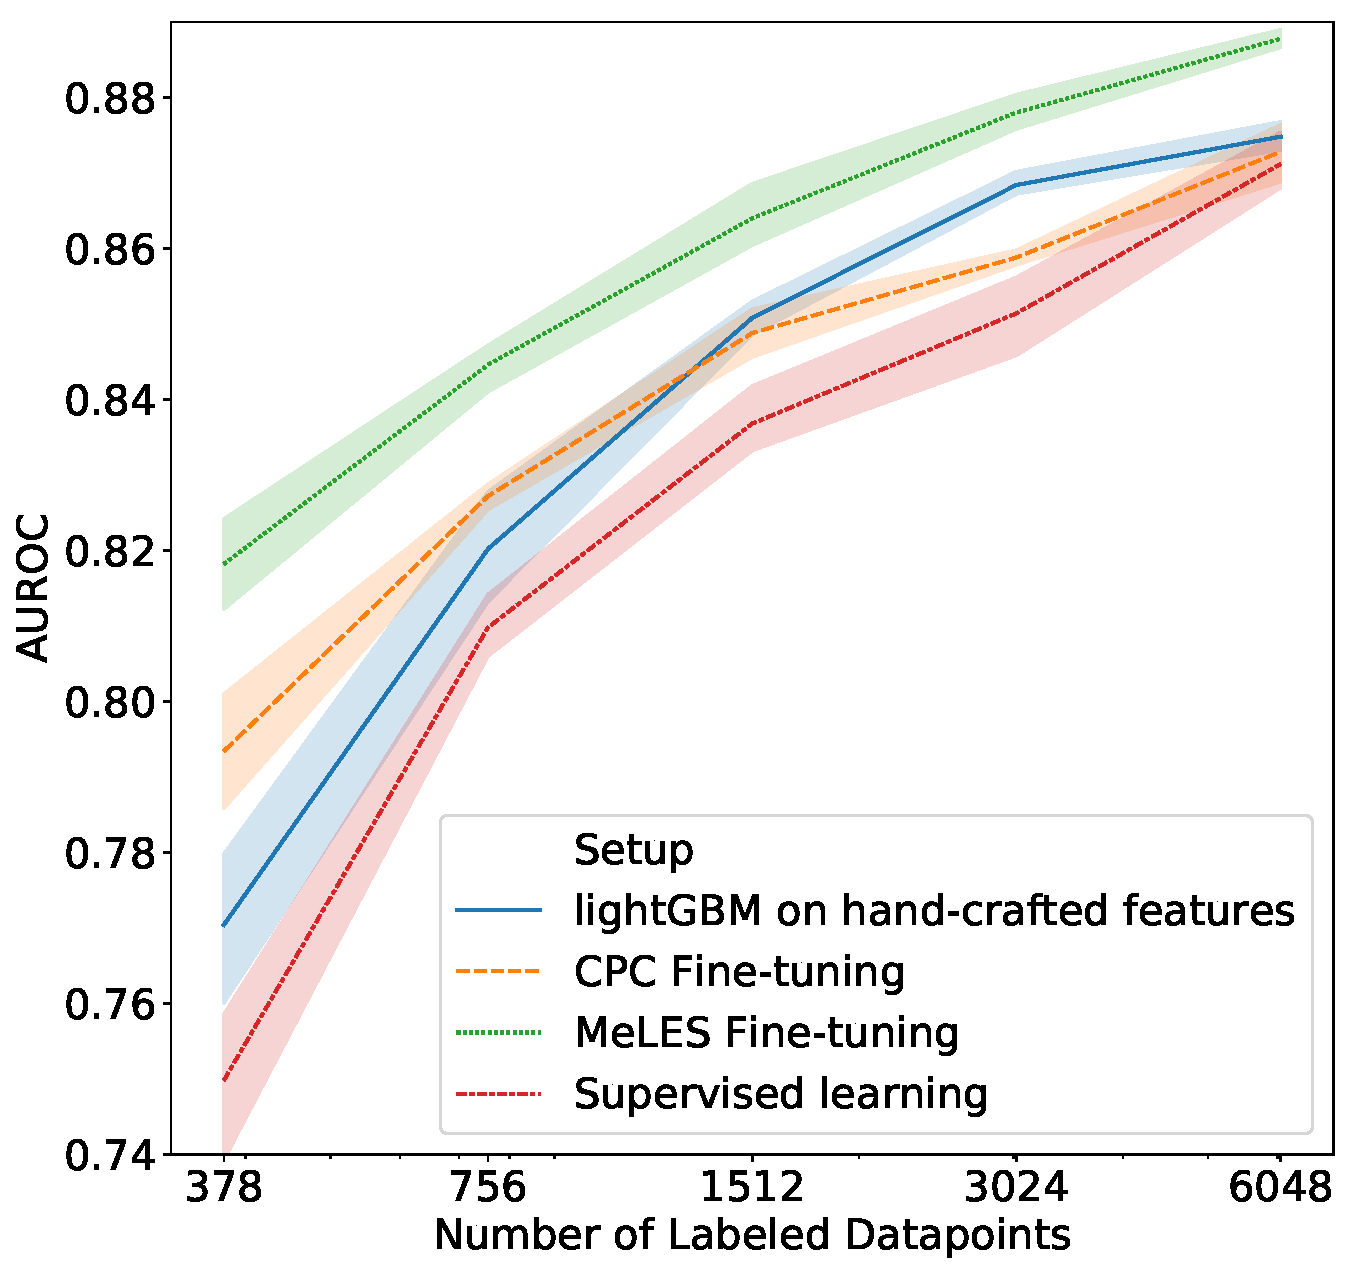
\includegraphics[width=\linewidth]{figures/ss_gen_4.pdf}
    \label{fig-semi-gender-0}
  \end{subfigure}
  \begin{subfigure}{0.5\linewidth}
    \caption{Assessment}
    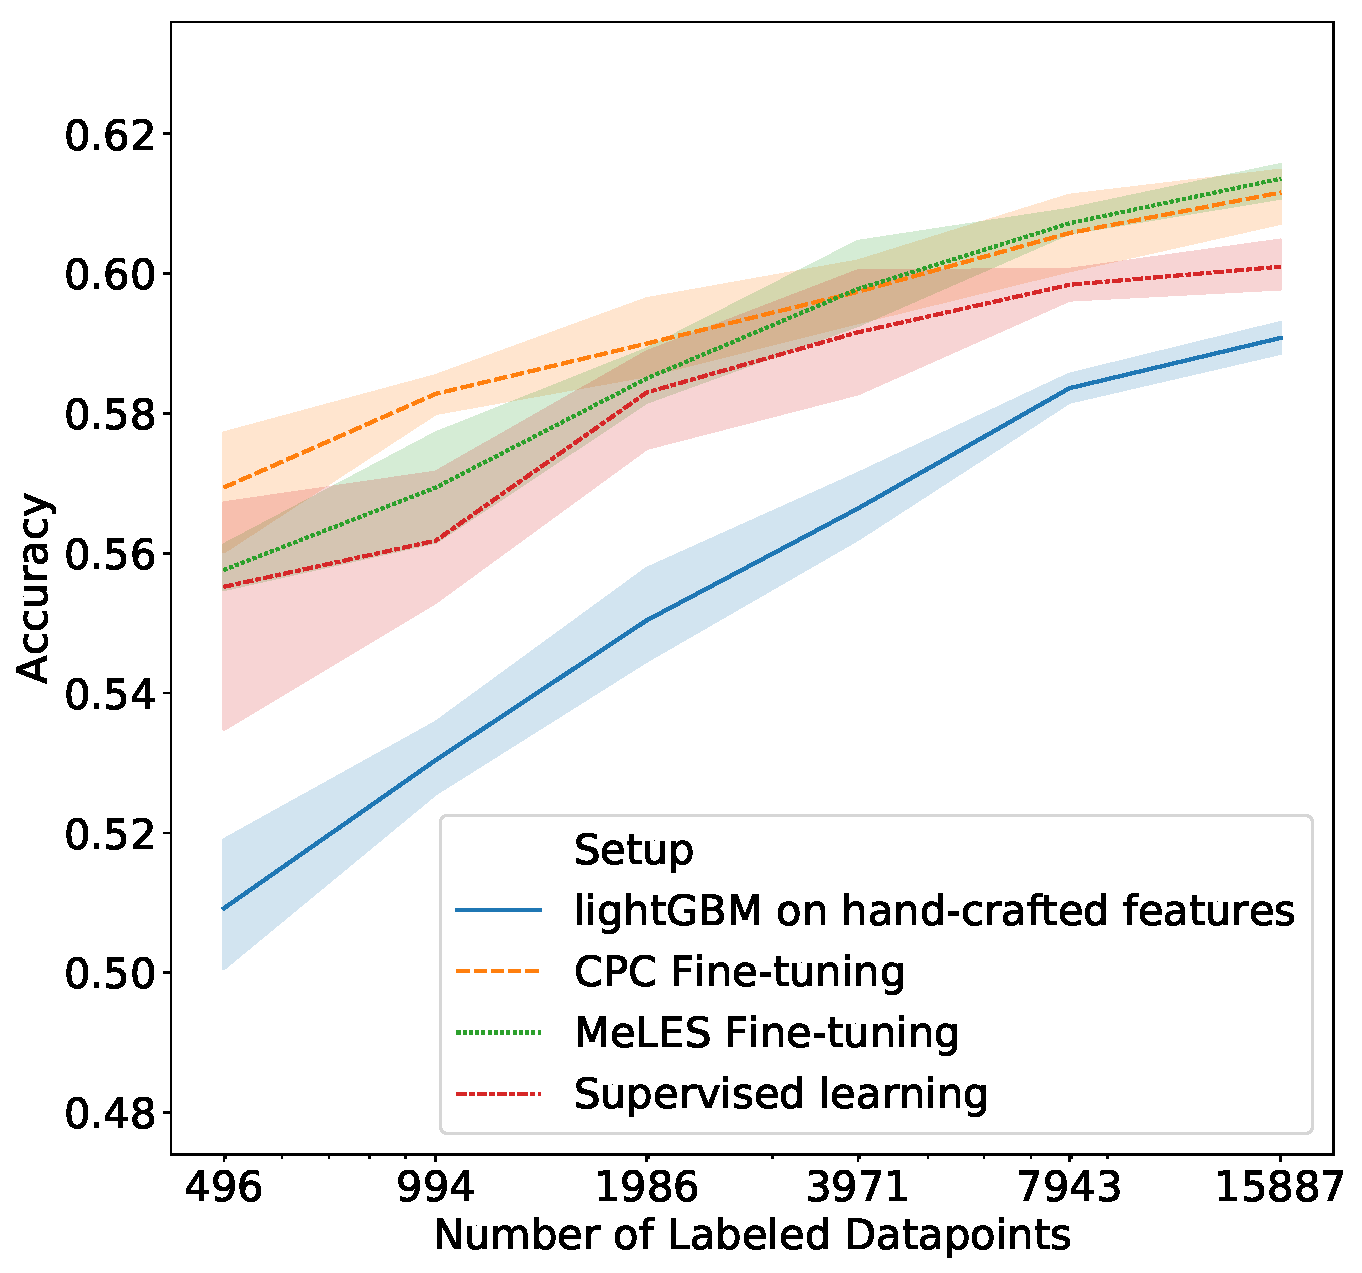
\includegraphics[width=\linewidth]{figures/ss_assessment.pdf}
    \label{fig-semi-age-1}
  \end{subfigure}%
  \begin{subfigure}{0.5\linewidth}
    \caption{Retail}
    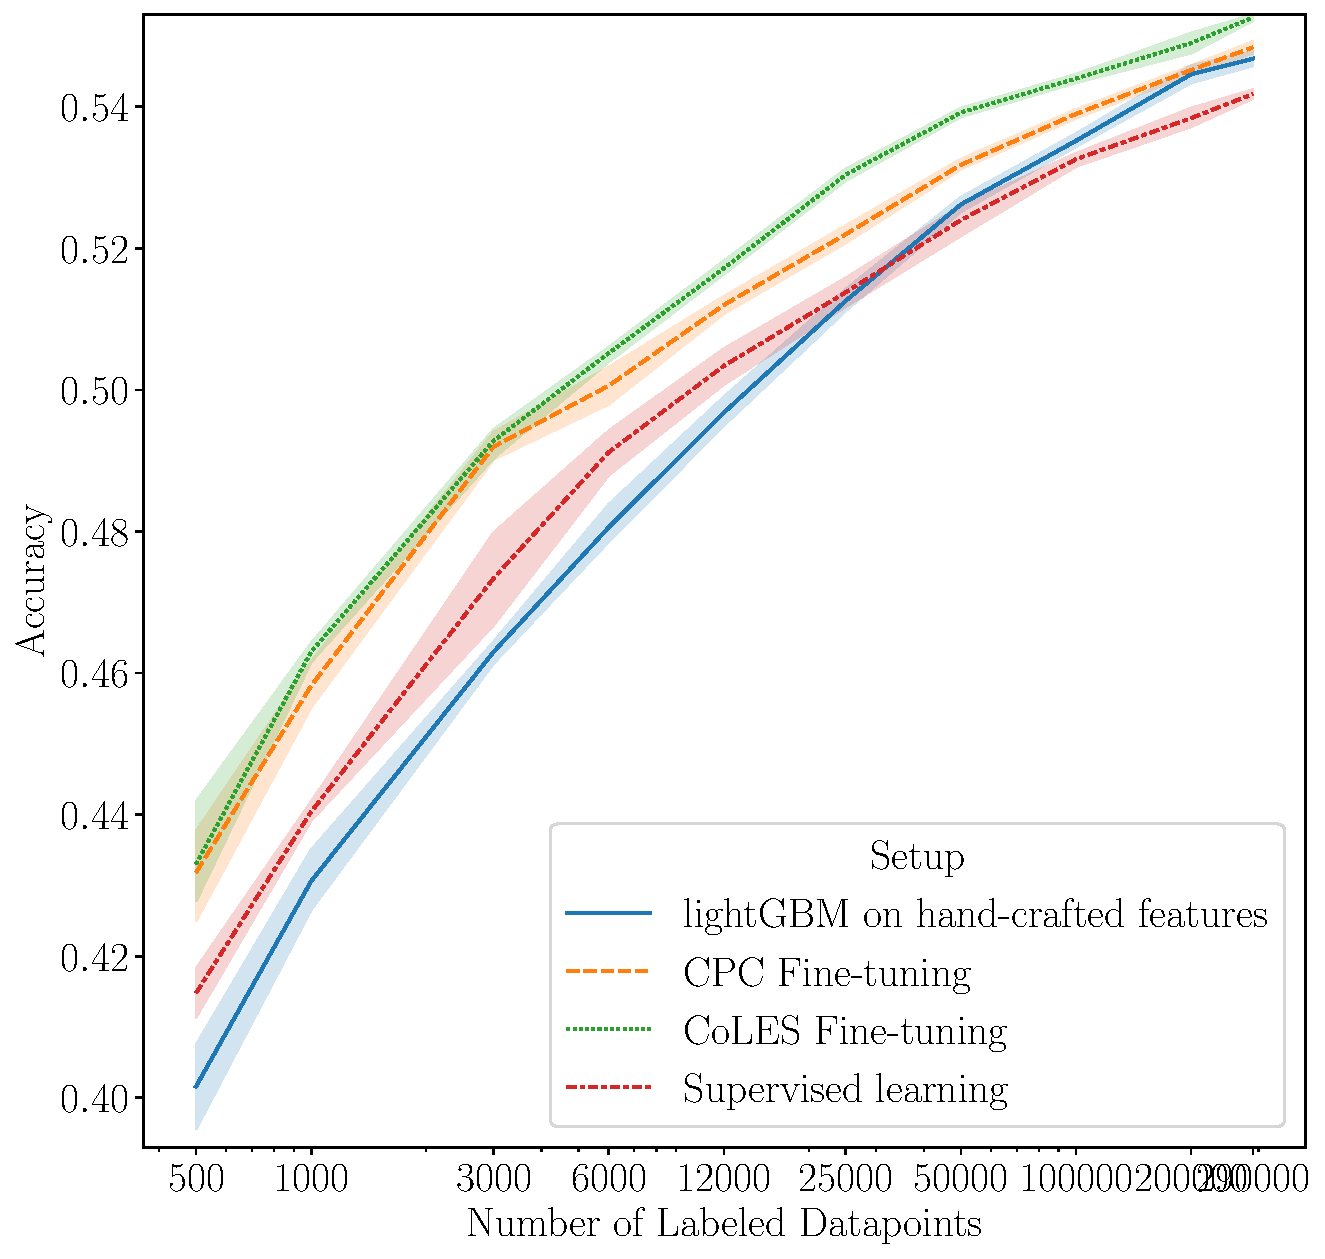
\includegraphics[width=\linewidth]{figures/ss_x5.pdf}
    \label{fig-semi-gender-1}
  \end{subfigure}
  \caption{Model quality for different dataset sizes} \small{The rightmost point correspond to all labels and supervised setup. X-axis is shown on a logarithmic scale.}
  \label{fig-semi}
\end{figure}

\subsection{Embedding visualization} \label{app-sec-vis}

In order to visualize MeLES embeddings in 2-dimensional space, we applied tSNE transformation~\cite{Maaten2008VisualizingDU} on them. tSNE transforms high-dimensional space to low-dimensional based on local relationships between points, so neighbour vectors in high-dimensional embedding space are pushed to be close in 2-dimensional space. We colorized 2-dimensional vectors using the target values of the datasets.

Note, that embeddings was learned in a fully self-supervised way from raw user transactions without any target information. Sequence of transactions represent user' behavior, thus the MeLES model captures behavioral patterns and outputs embeddings of users with similar patterns nearby.
As shown below, local clusters in embedding space correspond to distribution of user's attributes either age or gender.

tSNE vectors from the age prediction dataset are presented in the Figure \ref{fig-tsne-age2}. We can observe 4 clusters: clusters for group '1' and '2' are on the opposite side of the cloud, clusters for groups '2' and '3' are in the middle.

Taking into account that age is an ordinal attribute, we can make an assumption about the ordering of age groups: $age(1) < age(3) < age(0) < age(2)$ or vice versa. ($age(bin)$ returns age of user for specific group).

tSNE points from gender prediction dataset are presented in the Figure \ref{fig-tsne-gender2}. There are areas dominated by one gender label over another.

\begin{figure}
  \centering
  \caption{2D tSNE mapping of MeLES embeddings colored by target labels}
  \begin{subfigure}{0.5\textwidth}
    \caption{Age prediction}
    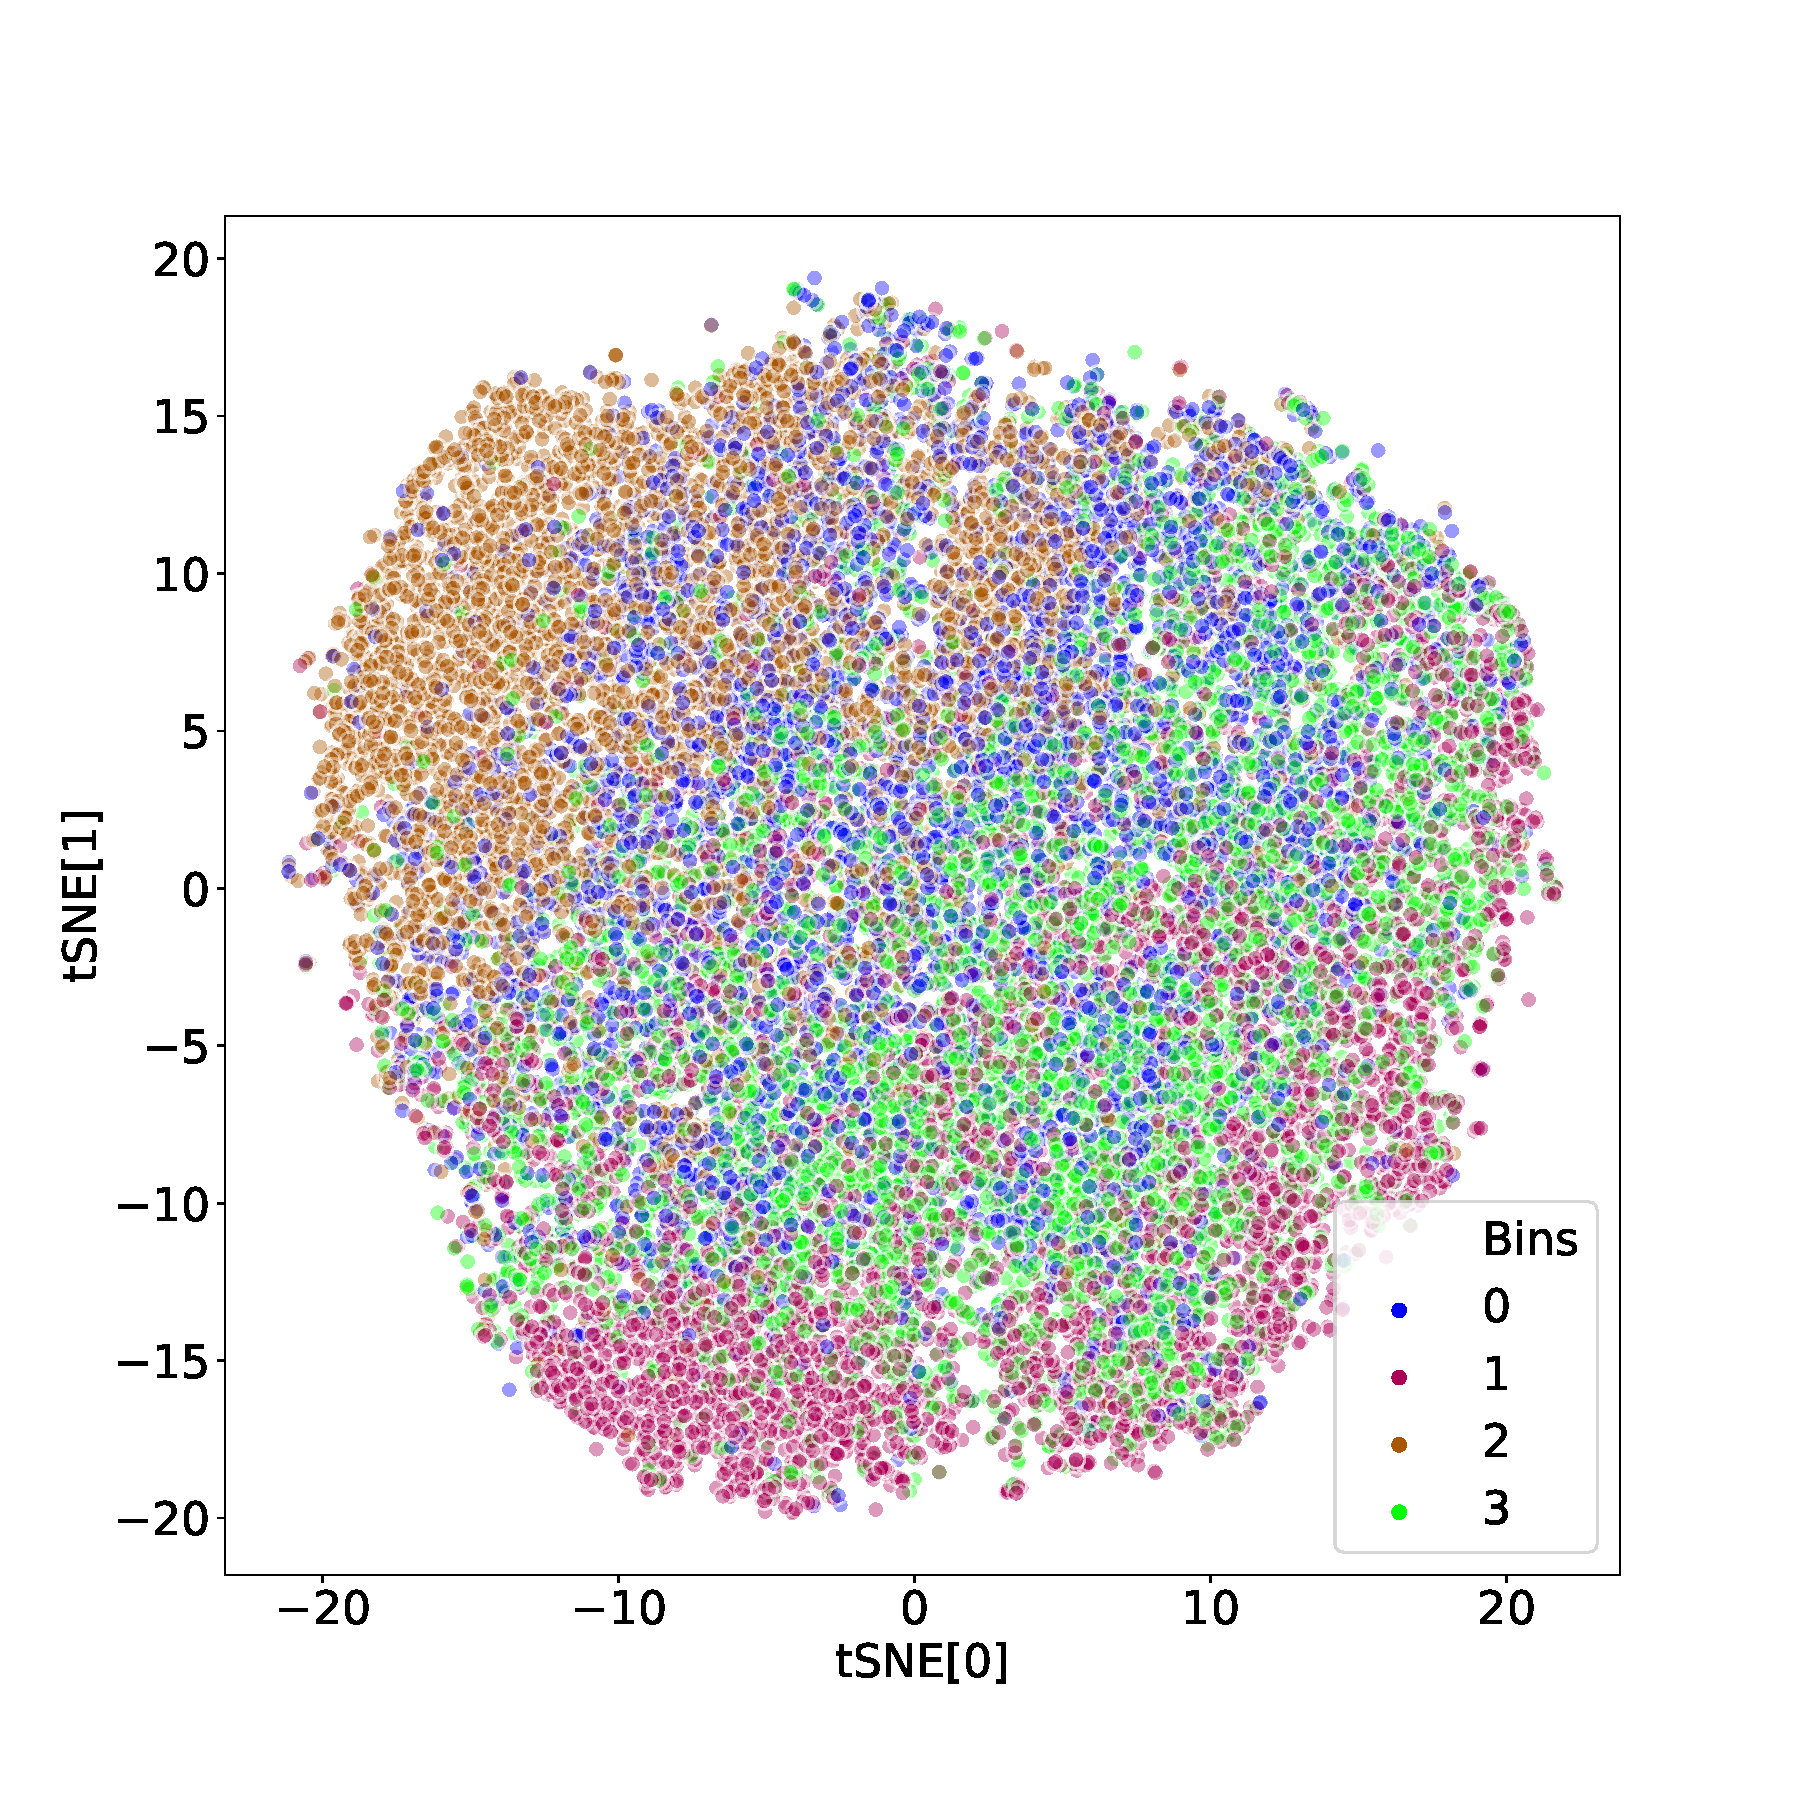
\includegraphics[width=\textwidth]{figures/age-pred-tsne2.pdf}
    \label{fig-tsne-age2}
  \end{subfigure}%
  \begin{subfigure}{0.5\textwidth}
    \caption{Gender prediction}
    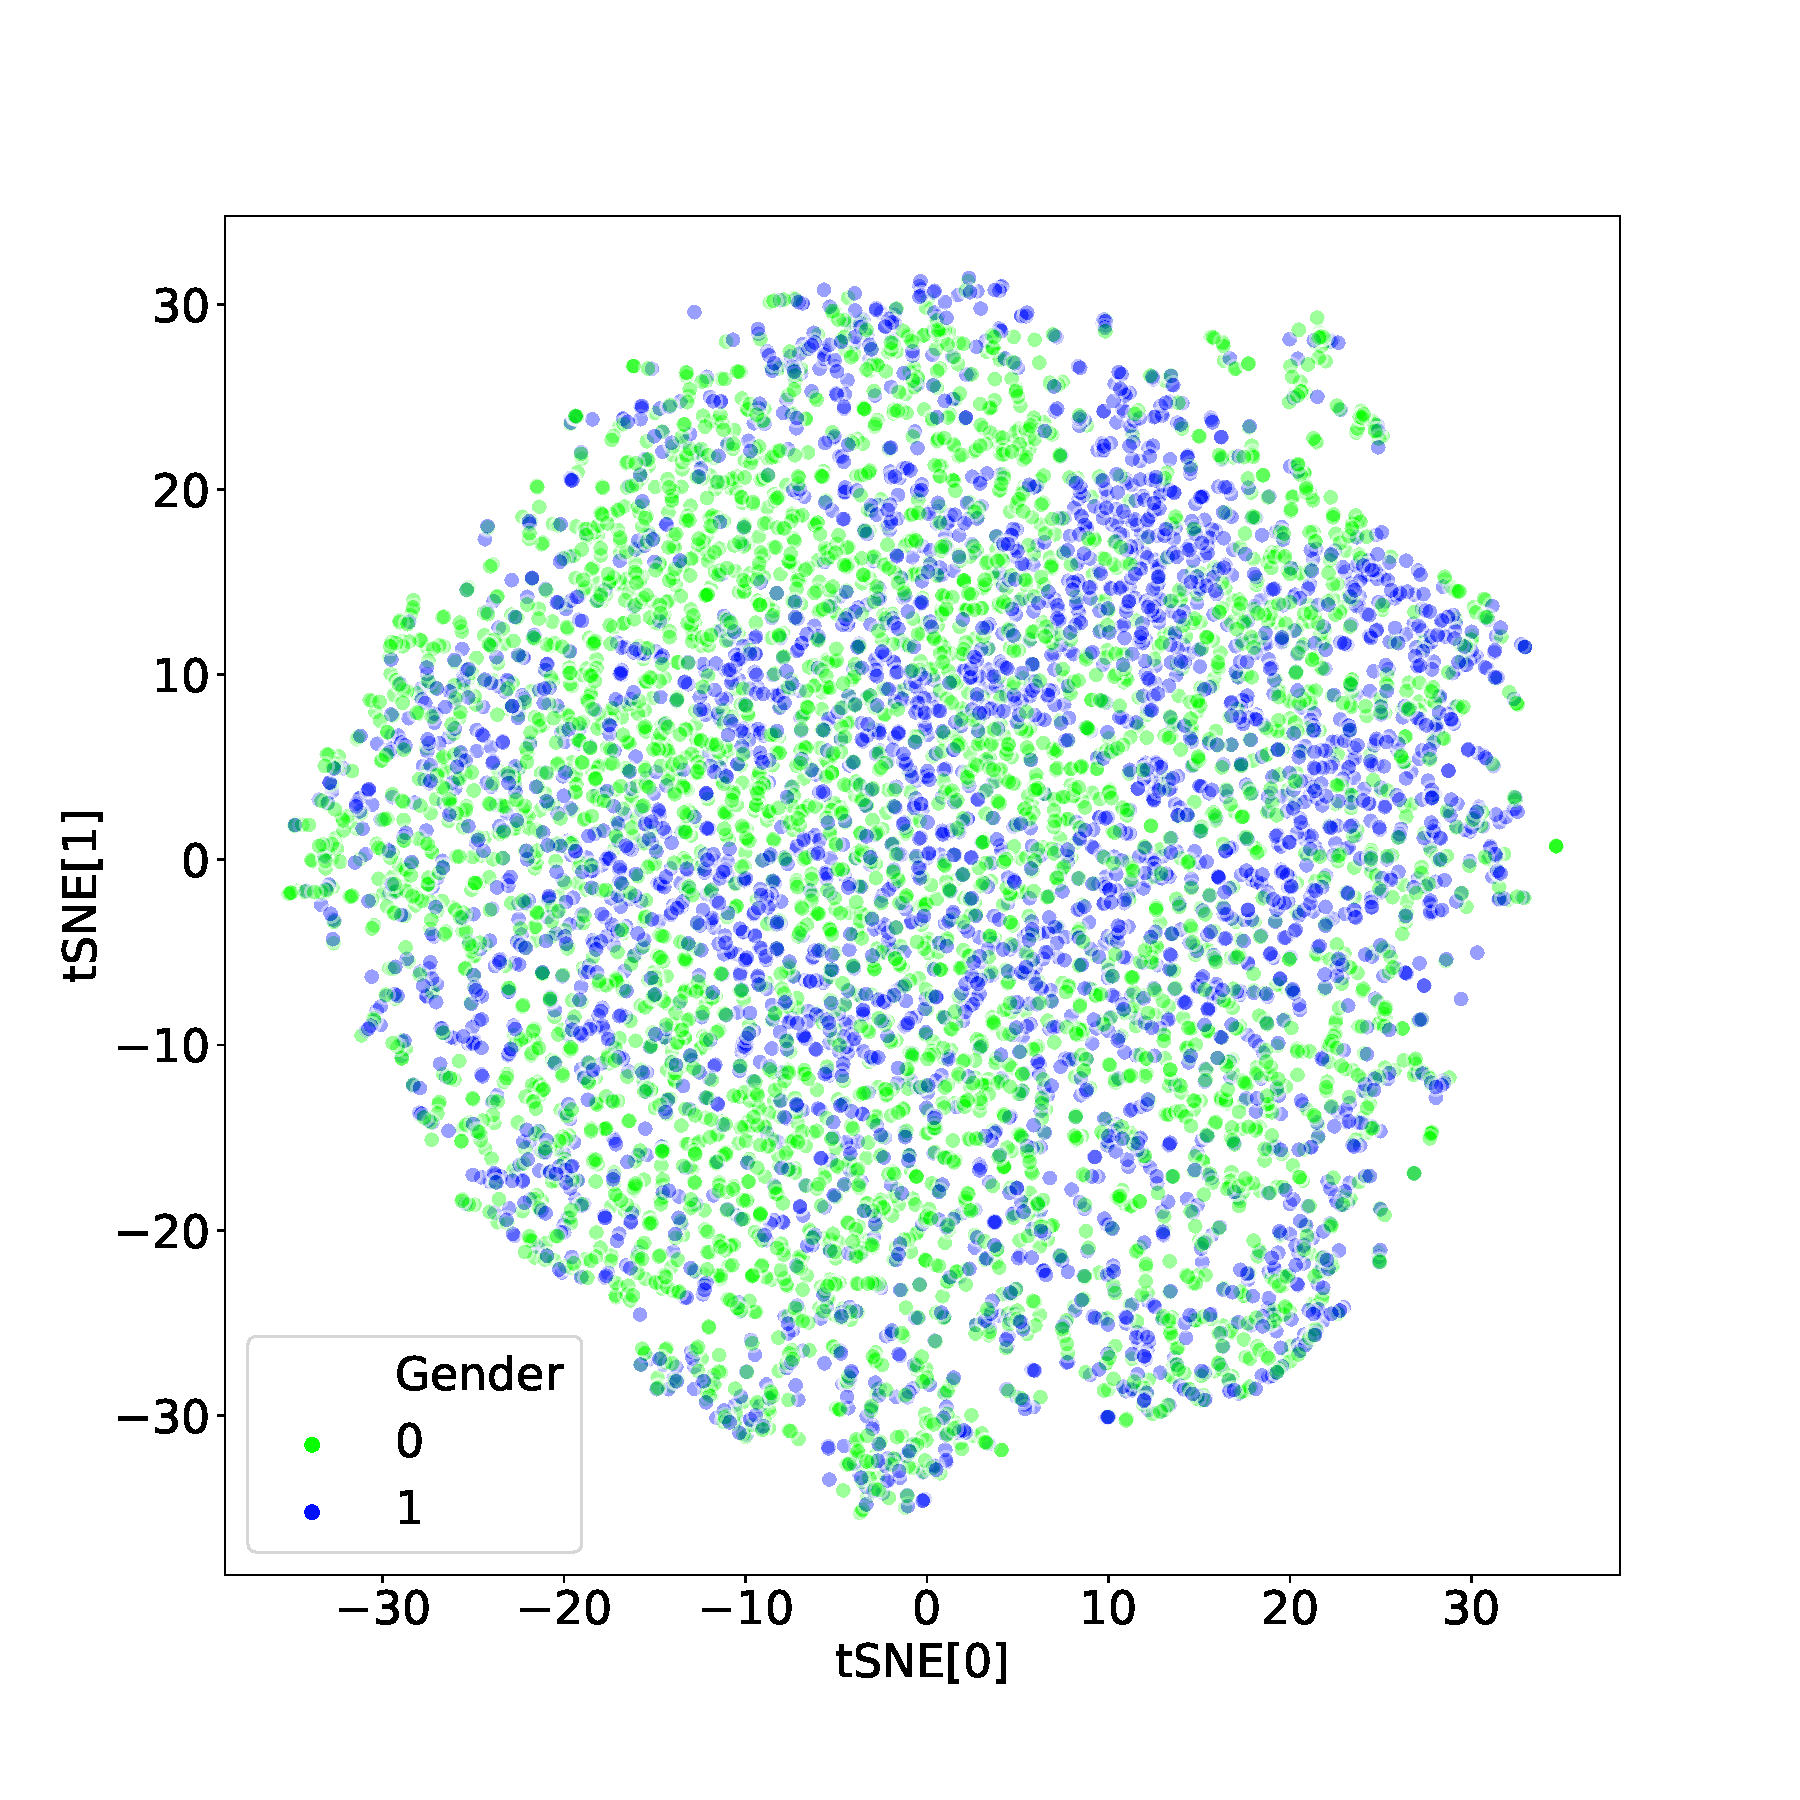
\includegraphics[width=\textwidth]{figures/gender-tsne2.pdf}
    \label{fig-tsne-gender2}
  \end{subfigure}

  \begin{subfigure}{0.5\textwidth}
    \caption{Assessment}
    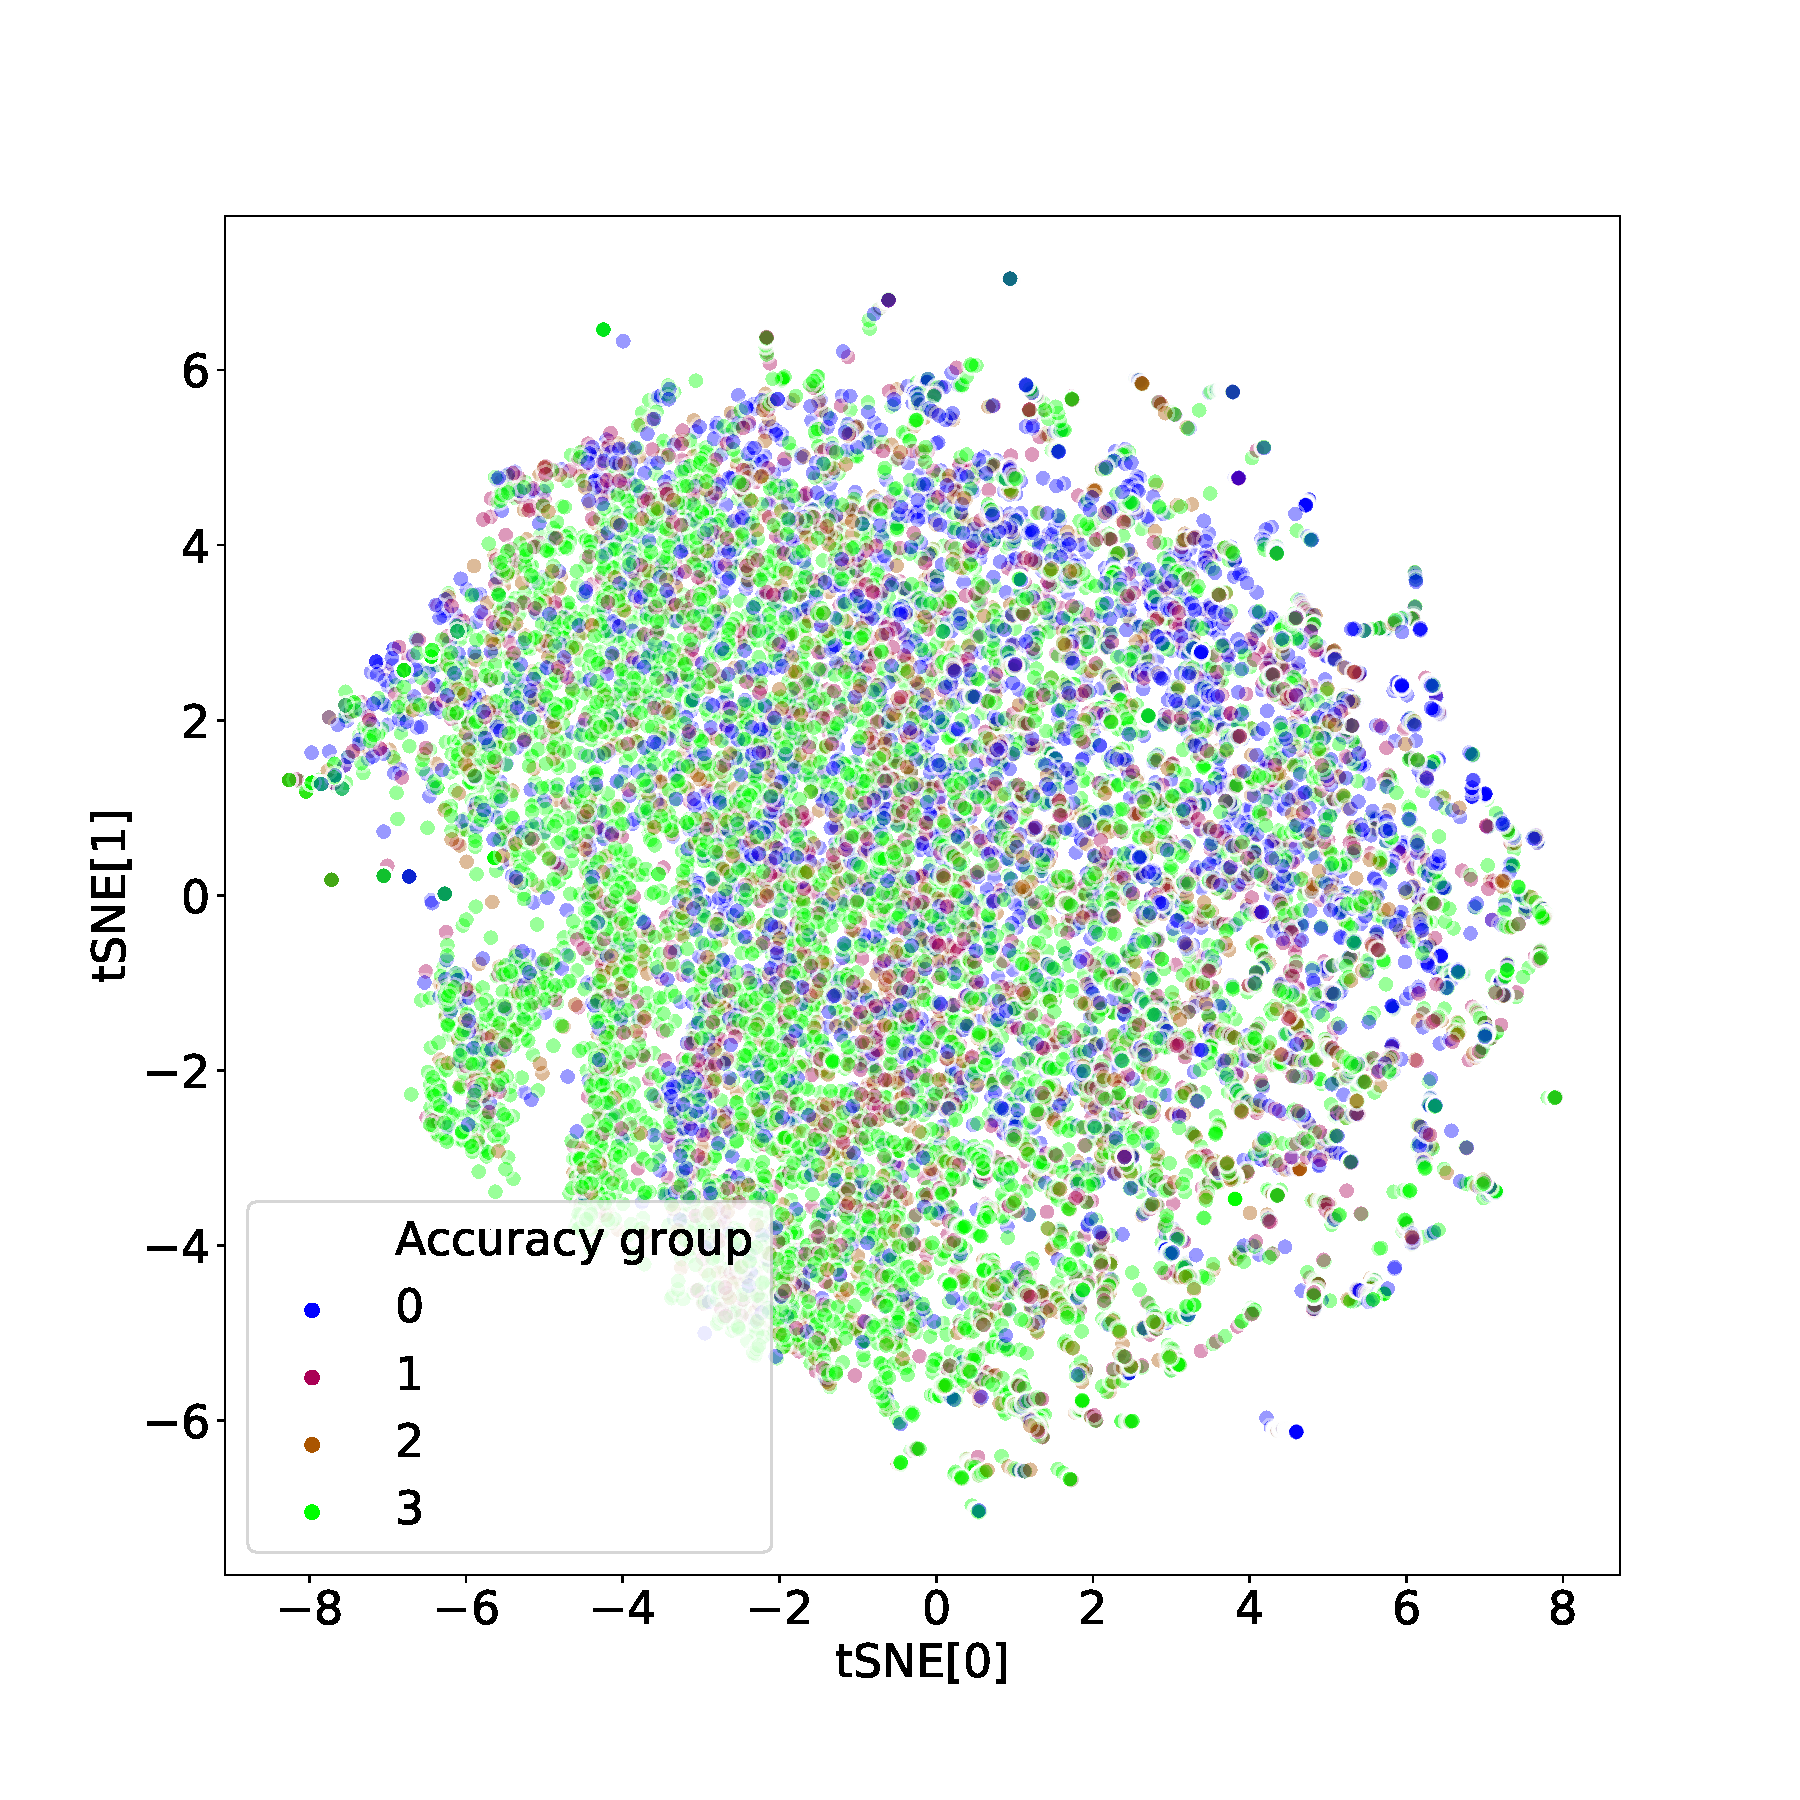
\includegraphics[width=\textwidth]{figures/bowl-tsne-accuracy_group.pdf}
    \label{fig-tsne-bowl}
  \end{subfigure}%
  \begin{subfigure}{0.5\textwidth}
    \caption{Retail}
    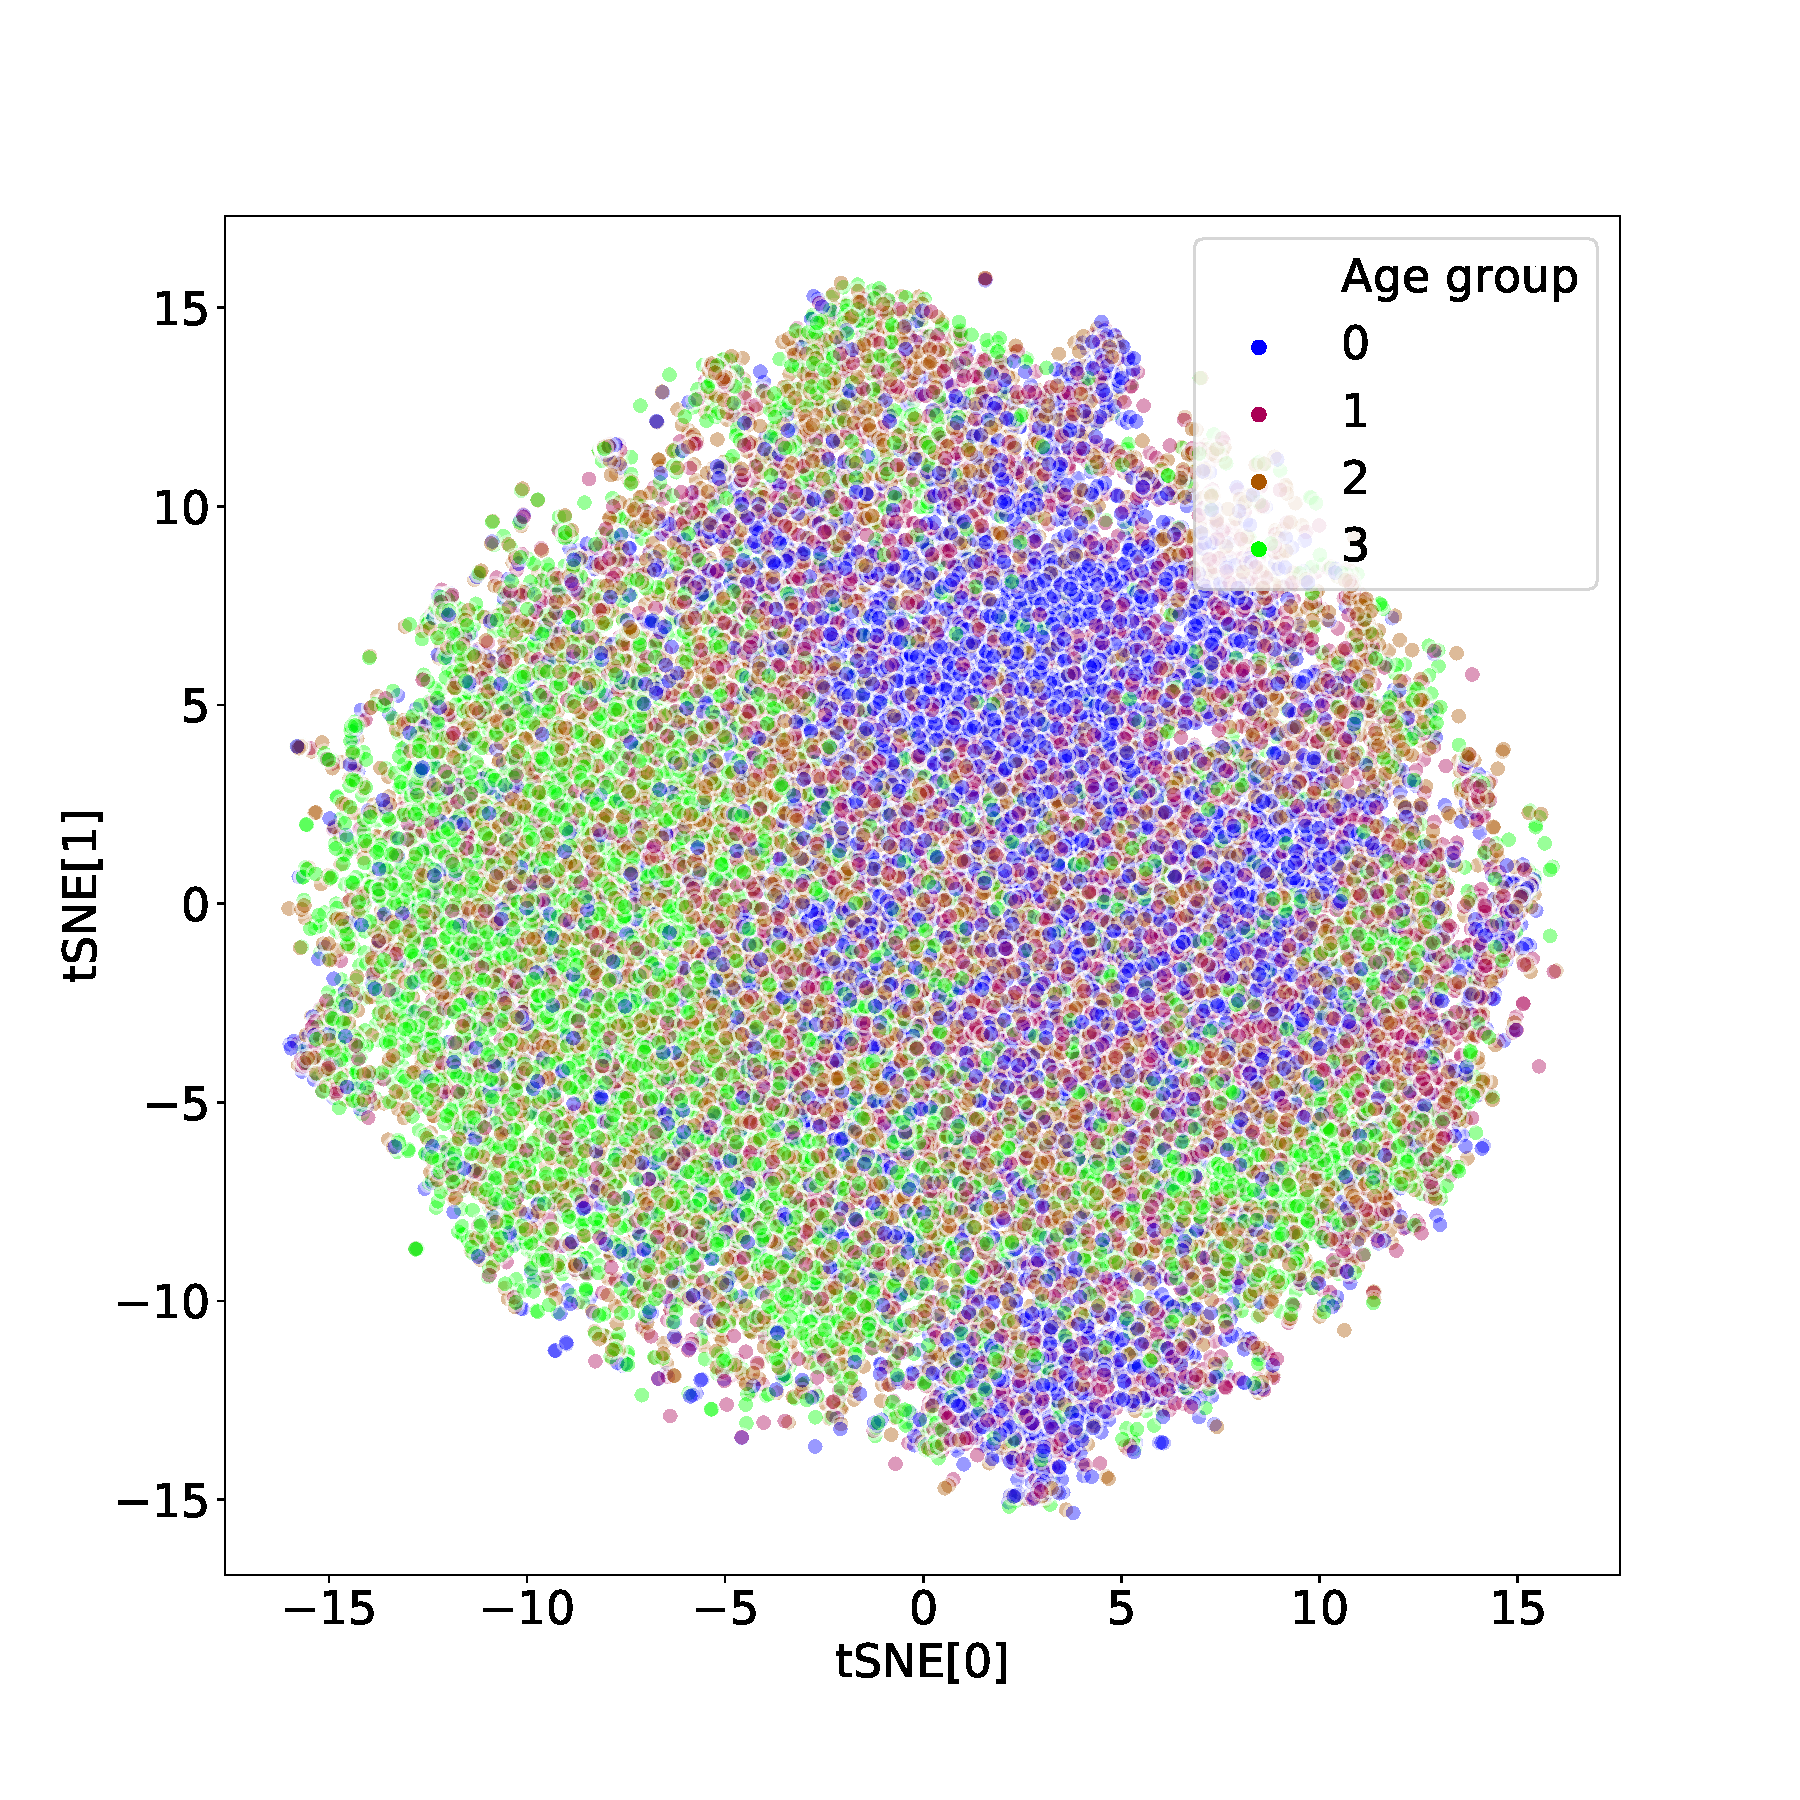
\includegraphics[width=\textwidth]{figures/x5-tsne-age_bin.pdf}
    \label{fig-tsne-x5}
  \end{subfigure}
\end{figure}

\end{document}
